\chapter{ConTrib: Maintaining Fairness in Decentralized Big Tech Alternatives by Accounting Work}
\label{chapter:trustchain}

\emph{\enquote{Big Tech} companies provide digital services used by billions of people.
Recent developments, however, have shown that these companies often abuse their unprecedented market dominance for selfish interests.
Meanwhile, decentralized applications without central authority are gaining traction.
Decentralized applications critically depend on its users working together.
Ensuring that users do not consume too many resources without reciprocating is a crucial requirement for the sustainability of such applications.}

\emph{In this chapter we present \TrustChain{}, a universal mechanism to maintain fairness in decentralized applications by accounting the work performed by peers.
In \TrustChain{}, participants maintain a personal ledger with tamper-evident records.
A record describes some work performed by a peer and links to other records.
Fraud in \TrustChain{} occurs when a peer illegitimately modifies one of the records in its personal ledger.
This is detected through the continuous exchange of random records between peers and by verifying the consistency of incoming records against known ones.
Our simple fraud detection algorithm is highly scalable, tolerates significant packet loss, and exhibits relatively low fraud detection times.
We experimentally show that fraud is detected within seconds and with low bandwidth requirements.
To demonstrate the applicability of our work, we deploy \TrustChain{} in the \Tribler{} file-sharing application and successfully address free-riding behaviour.
This two-year trial has resulted in over \TrialRecords{} records, created by more than \TrialUsers{} users.}

\newpage

\section{Introduction}

Over the last decades, \enquote{Big Tech} companies have obtained an unprecedented market dominance in the industry for information technology~\cite{frost2019bigtech}.
Companies such as Google, Amazon, Facebook, and Apple are omnipresent in our current society and even have the means of acting as small states, inhabited by billions of users worldwide.
By continuously broadening their activities, these companies seek to expand their virtual territory and seek to obtain monopolistic control over the enabling elements for digital services, such as access to the Internet~\cite{best2014internet}.

The societal impact of \enquote{Big Tech} companies is a double-edged sword.
On the one hand, these companies are facilitating new modes of digital interaction between users and enable new business models.
The sharing economy is a prime example of this phenomena.
It is made up by digital markets for the trustworthy exchange of personal assets (e.g., houses and cars) between strangers~\cite{schor2016debating}.
Sharing personal assets is a concept that has long been confined to trusted individuals, such as family and friends~\cite{frenken2019putting}.
Likewise, media platforms such as YouTube provide the required infrastructure for new forms of user engagement through video weblogging or \enquote{vlogging}.

On the other hand, it has become apparent that \enquote{Big Tech} companies tend to exploit their established market position and are increasingly involved in regulatory or political battles.
This behaviour sometimes goes undetected for years.
For example, researchers have only recently demonstrated that Uber actively manipulates the matchmaking process between passengers and drivers for commercial interests, therefore decreasing platform fairness and income equality of drivers~\cite{bokanyi2019ride}.
Similarly, Apple is currently under antitrust investigation by the European Commission that is assessing whether Apples' rules for developers on the distribution of apps via the App Store violate competition rules~\cite{kotapati2020antitrust}.

These concerning developments have contributed to an increase in the deployment of \emph{decentralized} applications.
Decentralized applications avoid centralized ownership and delegate the decision making away from a single authority.
A decentralized application mainly operates through the direct cooperation and information exchange between users, which we call \emph{peers}.
Arguably, Bitcoin is the most influential solution in this direction and provides a decentralized cash system without the supervision by an authoritative bank~\cite{nakamoto2019bitcoin}.
The underlying data structure of Bitcoin, a blockchain, is at the core of numerous decentralized applications~\cite{bashir2018mastering}.
At the time of writing, there are thousands of decentralized applications deployed on the Ethereum blockchain alone~\cite{wood2014ethereum}.
These decentralized applications include marketplaces, auctions, voting systems, lotteries, and games.

In contrast to the applications deployed by \enquote{Big Tech} companies, decentralized applications are fully maintained by peers, without coordination by a third party.
Decentralized applications require peers to pool their computer resources to provide the desired services to participants.
Specifically, peers have to communicate with other peers, have to dedicate computational power to process incoming network messages, and frequently have to store data generated by other peers.
Some decentralized applications critically depend on the voluntary contribution of computer resources by peers.
Bitcoin, for example, prevents the uncontrolled minting of digital coins through a resource-based consensus mechanism executed by miners~\cite{nakamoto2019bitcoin}.
These miners continuously attempt to solve a computational puzzle, a resource-intensive task that decides who can append transactions to the blockchain ledger.
Another volunteer-based application is Tor, providing anonymity by routing Internet traffic through user-operated relay and exit nodes~\cite{dingledine2004tor}.

Unfortunately, long-term cooperation between peers in decentralized applications is non-trivial to achieve.
Not rewarding peers for performing work can result in an unfair situation where peers enjoy the services provided by others, without contributing computer resources in return.
This detrimental behaviour, also called \emph{free-riding}, can degrade network health in the long term, as dedicated peers will ultimately leave~\cite{locher2006free}.
Measurements have shown that free-riding often prevails in cooperative applications such as BitTorrent and Tor~\cite{sirivianos2007free}.
Since the cooperation between peers is at the heart of decentralized technology, we argue that this form of fairness is a crucial requirement for \emph{any} decentralized application to ensure long-term sustainability~\cite{jelasity2004detection}.
With the renewed interest in decentralized alternatives for \enquote{Big Tech}, ensuring fairness in decentralized applications is a significant challenge.
%Blockchain technology addresses this issue by requiring peers to pay a transaction fee when issuing transactions.
%Yet, the detection of abuse is non-trivial since the relevant data might not be immediately available. % is dispersed across the network.
%However, the deployment of decentralized platforms poses new technical challenges that have to be addressed.
%These challenges include identity management, data availability, inducing cooperative behaviour amongst peers, and abuse management.

\begin{figure}[t]
	\centering
	\includegraphics[width=.9\linewidth]{trustchain/assets/trust_cycle}
	\caption{Addressing fairness issues in decentralized networks through work accounting, reputation and resource allocation. This work introduces a lightweight mechanism for secure work accounting.}
	\label{fig:trust_cycle}
\end{figure}

A promising approach to address these fairness issues is by deploying a decentralized reputation mechanism, and allocate resource based on trust scores of individuals.
This process is visualized in Figure~\ref{fig:trust_cycle}.
First, users account all performed and consumed work in the network within records.
A reputation mechanism then computes trustworthiness scores of users, based on created records.
A user decides who to help based on a resource management algorithm.
In general, users with low reputation scores should be refused services whereas trusted users enjoy preferential treatment from others.
There currently is no accounting mechanism that is specifically built to account work performed and consumed by peers in decentralized networks, to the best of our knowledge.

%Since an operator has access to all historical events in a centralized system, detecting and addressing the abuse of resources is straightforward to achieve.
%This is more challenging in decentralized systems since information is dispersed across the network.

%\todo{bash centralized gatekeepers + antitrust}
%As a counterforce to the centralized architectures deployed by big tech companies, there has been significant effort to deploy decentralized systems that avoid third-party supervision.
%Blockchain technology, for example, empowers participants with a distributed ledger to securely record interactions and has been a key enabler of numerous decentralized systems like Bitcoin and Ethereum.
%Whereas the deployment of centralized systems is relatively straightforward, decentralized systems usually require additional complexity to mitigate the threats commonly found in decentralized networks.
%Significant research challenges include data availability and trust management.
%These threats include data unavailability, free-riding, and the Sybil Attack.

%\todo{alternative solution -> most feasible one is decentralized}
%\todo{prevent abuse in decentralized systems}

%At the heart of many systems, both centralized and decentralized, lies a mechanism for the secure storage and management of user-generated data.
%The storage and management of information in a decentralized system is a long-standing research challenge.
%Centralized service providers like Facebook and Amazon store all user data is stored on one or multiple servers that are fully under the control of the platform operator.
%On the other hand, secure and robust data management is considerably more challenging in decentralized networks where data must be stored by other, possibly untrusted peers.

%, with varying degrees of adoption.
%Perhaps the most influential example is Bitcoin, a digital currency that is fully maintained by its participating users.
%Bitcoin has demonstrated that it is possible to build a coin without banks.
%The core technology of Bitcoin, the distributed blockchain ledger, has bootstrapped much interest in decentralized alternatives.\todo{for example?}
%Another example is BitTorrent, a decentralized file-sharing protocol that enables users to directly exchange information.



%One might leverage blockchain technology to decentralized information management.
%Blockchain enables the tamper-proof and irrefutable storage of generic data elements, usually represented as transactions.

%Many of these innovations are pioneered by blockchain technology, which has been hailed as a panacea to disrupt these developments.
%Specifically, blockchain technology empowers users themselves to take on critical roles that are traditionally fulfilled by trusted authorities, e.g., banks, reshaping the notion of interactions in our society.
%Despite thriving ecosystems and markets worth billions of dollars (e.g., Ethereum), the first use case to pose a real threat to big tech companies has yet to be.
%This lack is mainly addressed to scalability limitations: blockchain technology is not performant enough yet to capture financial transactions on a global scale.

% The key challenge is to build a fully decentralized system, fully maintained by individuals. Requires adequate fraud prevention + free-riding prevention.

% One paragraph explaining how accounting in big-tech alternatives is different from existing work (e.g., PeerReview, Lifting, ...)

% Argue about fairness?
% https://pdf.sciencedirectassets.com/272436/1-s2.0-S1084804516X00185/1-s2.0-S1084804516302788/main.pdf

\textbf{Our Solution.}
We specifically focus on the accounting of work performed by peers, which is crucial to ensure fairness within decentralized applications.
In this work, we design, implement and evaluate a universal data store, named \TrustChain{}.
\TrustChain{} is capable of accounting work within different decentralized applications.
Examples of work include storing files on behalf of other peers, performing computations, or relaying network packets.
With \TrustChain{}, each peer maintains a \emph{personal ledger} with tamper-evident \emph{records}.
The \TrustChain{} records can then be used by an application to determine the trustworthiness of individuals, e.g., with a reputation algorithm.
Consequently, users have a natural incentive to increase their social standing by modifying or removing records.
This misbehaviour is a key threat to the integrity of the \TrustChain{} data structure.
We refer to the illegitimate modification of a record as fraud.
To detect fraud, peers continuously request random records from other peers and disseminate newly created records in the network.
Peers verify the consistency of incoming records with the ones stored in their database.

\begin{figure}[t]
	\centering
	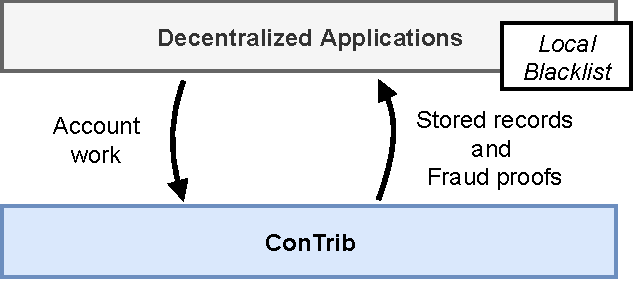
\includegraphics[width=.6\linewidth]{trustchain/assets/contrib_app_interaction}
	\caption{Decentralized applications can use \TrustChain{} to account the work performed by peers within tamper-evident \emph{records}. These records are used by connected applications to detect free-riders and fraudsters, which are added to a local blacklist. Applications can then choose to refuse services to the peers on the blacklist.}
	\label{fig:interaction_with_apps}
\end{figure}

\TrustChain{} enables connected applications to select which work should be accounted.
Figure~\ref{fig:interaction_with_apps} shows how a decentralized application can leverage \TrustChain{} to account work.
By inspecting the records in personal ledgers, an application can gather evidence of free-riding behaviour.
Each application maintains a local blacklist with both free-riders and peers that have committed fraud.
Peers refrain from performing work for peers on the blacklist.
\TrustChain{} can be deployed to alleviate fairness concerns in a wide range of decentralized applications, including peer-assisted video distribution, anonymous communication networks, and distributed learning environments.

We implement \TrustChain{} and evaluate how different parameters impact the efficiency of fraud detection and the network usage.
We find that fraud can be detected within seconds on average, even in larger networks with 10'000 peers where every peer commits fraud, and under a conservative strategy for record exchange.
We also show that \TrustChain{} highly tolerates packet loss.

To show the effectiveness of \TrustChain{} in a realistic environment, we employ our accounting mechanism to address free-riding behaviour in \Tribler{}.
\Tribler{} is a decentralized application downloaded by over 1.7 million users~\cite{pouwelse2008tribler}.
We specifically use \TrustChain{} to account bandwidth exchanges in \Tribler{}s' Tor-like overlay and use the accounted work to refuse services to free-riders.
Our two-year measurements have resulted in over \TrialRecords{} records, created by more than \TrialUsers{} users.
This large-scale deployment trial is a key milestone in our ongoing research effort to solve the tragedy-of-the-commons within Internet communities~\cite{de2018blockchain}.

The main contribution of this work is four-fold:
\begin{enumerate}
	\item \TrustChain{}, a \emph{universal mechanism} that maintains fairness in decentralized applications by accounting work (Section~\ref{sec:micro_accounting}).
	\item An efficient \emph{fraud detection mechanism} to detect the illegitimate tampering of created records in \TrustChain{} (Section~\ref{sec:detecting_fraud}).
	\item An \emph{implementation} and \emph{evaluation} of \TrustChain{} with up to 10'000 peers, demonstrating the scalability of our mechanism and showing that fraud can be detected within seconds on average (Section~\ref{sec:system_architecture} and Section~\ref{sec:implementation_evaluation}).
	\item A \emph{two-year deployment trial} of \TrustChain{} in \Tribler{}, involving \TrialUsers{} Internet-recruited volunteers. This trial successfully addresses free-riding behaviour in \Tribler{} (Section~\ref{sec:deployment}).
\end{enumerate}

% We introduce ...

% Collective memory ...

%\section{Introduction}
%Free-riding, the act of selfishly benefiting from the usage of shared resources, is a common issue in both real-world and Internet communities~\cite{rose2003internet,adar2000free}.
%This selfish behaviour frequently prevails in Internet communities.
%This behaviour occurs when access to a shared resource is cheap and there are no individual consequences of overusing the good by community members.
%Structural free-riding on collective resources may result in a \emph{tragedy-of-the-commons}, the situation in shared-resource systems where the resource is depleted and the community around the resource collapses~\cite{hardin2009tragedy}.
%In this work, we address this behaviour by introduce a mechanism for digital shared-resource systems where all resource contributions and consumptions are accounted.
%Free-riding is a prevalent strategy within Internet communities.
%For example, digital media is aggressively competing for user attention, a scarce resource, through the unsolicited presentation of invasive banner ads and clickbait articles~\cite{chen2015misleading}.
%Ongoing Denial-of-Service (DOS) attacks on specific machines is another example of free-riding and shows that some individuals selfishly exploit the ubiquitous access to the Internet~\cite{cerf2013revisiting}.
%This behaviour shows that these attackers have a stronger incentive to undermine the security of shared Internet resources, rather than contributing to it.

%Shared-resource systems on the Internet are vulnerable to free-riding behaviour~\cite{locher2006free}.
%These systems are managing individuals with mutual access to computer resources offered to the community (e.g., bandwidth or CPU capacity).
%For example, downloading in the BitTorrent file-sharing network without contributing (seeding) back after the download has finished goes mostly unpunished and is therefore a common strategy~\cite{locher2006free}.
%Free-riding also occurs in anonymous networks like Tor, where users free-ride on the services offered by relay and exit nodes, without offering community services in return.
%Failure to acknowledge the presence of free-riding behaviour in peer-to-peer networks degrades the systems performance and could eventually result in users permanently leaving the network, as illustrated by the Gnutella software~\cite{adar2000free}.

%To date, the \emph{tragedy-of-the-commons} in Internet communities remains unsolved~\cite{harris2018institutional}.
%This social dilemma occurs where the community around a shared resource, e.g., storage capacity or bandwidth, will eventually collapse due to overexploitation when individual self-interest is at odds with community interests.
%A well-known example is \emph{free-riding} in file-sharing networks, where the act of downloading content without contributing (seeding) back after the download has finished goes mostly unpunished~\cite{locher2006free}.
%Long-term non-cooperative behaviour in shared-resource systems degrades the network performance and eventually leads to a community collapse as illustrated by peer-to-peer applications like  Gnutella~\cite{adar2000free}.

%The Internet has turned into a grim place, where selfish interest of big tech companies supersedes the importance of user-managed communities.
%Email spam is a prominent example of what happens when bandwidth is abused for selfish reasons.
%Over 45\% of email traffic consists of junk messages and an increasing number of ISPs and hosting providers are being forced to use sophisticated techniques in order to try at least to reduce it.
%Likewise, digital media is competing for user attention through the unsolicited presentation of invasive banner ads and clickbait articles.
%Ongoing DDoS attacks on specific machines show that some individuals have a stronger incentive to undermine the security of the Internet, rather than contributing to it.



%Oftentimes, the allocation of shared resources such as bandwidth is prescribed by the output of an algorithm that considers all historical contributions and consumptions of a peer~\cite{tang2004trust}.
%This trust can be based on historical action, or on a believe that the other agent will reciprocate a service later.
%Trade-based incentive mechanisms rely on remuneration for the volunteer resource sharing by agents, either through credits or monetary value.
%This is the approach taken by volunteer computing services, e.g., Boinc, and blockchain-based resource markets, e.g., FileCoin~\cite{benet2018filecoin} and Orchid~\cite{cannellorchid}.

%Providing meaningful incentives to reciprocate after taking some of its resources is imperative to alleviate free-riding behaviour and boost cooperating amongst participants~\cite{ma2004incentive}.
%Some shared-resource systems rely on a \emph{trade-based incentives} where resource consumption is immediately remunerated using a credit or payment system.
%For example, in many volunteer computing projects offered by BOINC users are rewarded for their contributed resources with virtual credits.
%Likewise, shared-resource systems build on blockchain technology leverage cryptocurrency payments to reward communal services~\cite{benet2018filecoin}.

%With \emph{trust-based incentives}, community members are indirectly reciprocated.
%Usually, the amount of provided and consumed resources to and from the community is expressed in a trust score, which can be computed by a reputation mechanism~\cite{meulpolder2009bartercast}.
%These scores are then used to determine a fair allocation of resources, for example, peers with a higher reputation are granted preferential treatment during periods of congestion.
%These trustworthiness scores can be computed by a reputation algorithm.
%To accurately determine the trustworthiness of individuals, shared-resource systems require a public accounting mechanism that records all interactions between users.
%This work focusses on secure accounting of interactions in such systems.

%There have been several proposals to address free-riding behaviour by securely accounting interactions~\cite{guerraoui2010lifting,haeberlen2007peerreview,mokhtar2014acting}.
%We find, however, that existing work is lacking in two directions.
%First, the design of existing solutions usually considers a specific application, e.g., file-sharing or gossip networks.
%This makes it hard, if not impossible, to re-use these solutions across shared-resource systems with differing resource types.
%Second, existing solutions tend to elevate the authority of specific peers in the network, e.g., by having a user act as witness for others.
%This introduces additional system complexities, e.g., incentivize users to not abuse their authority and to follow the protocol.

%As research points out, the interactions in digital shared-resource systems are usually short-lived and concern a small amount of resources~\cite{seuken2014work}.
%For example, the storage protocol FileCoin~\cite{benet2018filecoin} splits data into many small pieces and remunerate peers for the retrieval of individual pieces.
%Similarly, the BitTorrent file-sharing protocol orients around the transport of small data pieces with a variety of peers.
%Repeated, small interactions allows for lower risk-taking since peers can abort an interaction when its counterparty defects, e.g., when a counterparty goes offline during a file exchange.


%This approach aligns well with existing shared-resource systems where interactions are short-lived and concern a small amount of resources~\cite{seuken2014work}.
%For example, blockchain-based storage networks like FileCoin~\cite{benet2018filecoin} split data into small pieces and remunerate peers for the retrieval of pieces.
%Furthermore, micro-accounting allows for low risk-taking since peers can abort an interaction when its counterparty defects, e.g., when a counterparty goes offline during a file exchange.


%In this work, we design, implement, deploy and evaluate a 
%We identify two key advantages of micro-accounting

%So far, there is no lightweight and reusable \emph{micro-accounting} mechanism, specifically designed for recording small interactions in large shared-resource systems.

%Currently, there is no lightweight mechanism for tamper-proof accounting of community interactions, to the best knowledge of the authors.

% Motivate the need for micro-accounting
% 1) it aligns well with existing systems, e.g., file sharing and bandwidth sharing
% 2) it allows for quick punishment and blacklisting of users, with low value-at-risk

%So far, there has been a wide range of research in designing incentive-compatible mechanisms to prevent free-riding in decentralized networks.
%Many of the proposed models and mechanisms require secure accounting of community contributions, for example, if a peer has donated some storage to a specific peer or has uploaded a file to others.

%Most of these efforts are concentrated on reducing free-riding behaviour in file-sharing communities.
%However, free-riding is also prevalent in other communities, such as anonymity networks~\cite{biryukov2015proof}.
%We also observe that most research in this direction take a clean-slate approach for the implementation of their mechanisms.
%This leads to a large range of different implementations.
%Specifically, there is no universal, resource-agnostic infrastructure to quickly evaluate new mechanisms and policies.
%We argue that furthefr research on the management of Internet commons benefits from such an infrastructure.
%Many of these solutions share commonalities in the infrastructure required to deploy these mechanisms.

%\begin{figure}[b]
%	\centering
%	\includegraphics[width=\linewidth]{assets/components}
%	\caption{Our model for trust-based management of shared Internet resources such as bandwidth and storage.}
%	\label{fig:model}
%\end{figure}

%\begin{figure}[t]
%	\centering
%	\includegraphics[width=\linewidth]{assets/trust_cycle}
%	\caption{Our envisioned approach to address free-riding behaviour in large-scale shared-resource systems.}
%	\label{fig:trust_cycle}
%\end{figure}

%We present \TrustChain{}, a universal accounting mechanism for the detection of free-riding behaviour in shared-resource systems.
%Our mechanism enables resource accounting where fraud, e.g., illegitimate tempering of micro-records, can be efficiently detected across different shared-resource applications.
%\emph{Micro-records} are the key building block of \TrustChain{} and are linked together in a personal ledger.
%A micro-record describes an interaction from the perspective of one of the involved parties.
%Users continuously share micro-records with random users and validate incoming micro-records against known ones.
%Our simple, yet effective technique enables quick detection of fraud, specifically the situation where an adversary has forked its personal ledger.
%We implement \TrustChain{} and systematically evaluate its scalability and resistance against malicious users that undermine the accounting mechanism, e.g., by hiding or modifying the micro-records in their personal ledger.
%Our experiments with up to 1'000 users reveal that \TrustChain{} that fraud can be detected well within a minute and that the throughput of \TrustChain{} scales linearly with the network size.

%To show the effectiveness and matureness of \TrustChain{} in a realistic environment, we leverage our mechanism to record bandwidth traffic in \Tribler{}.
%\Tribler{} is our academic peer-to-peer software and downloaded by over 1 million users.
%Specifically, we use \TrustChain{} to account bandwidth exchanges in our Tor-like overlay and refuse services to free-riders during periods of congestion.
%Our 36-months measurements has resulted in over 120 million micro-records, created by over \TrialUsers{} users.
%This large-scale deployment trial is a key milestone in our ongoing research to solve the tragedy-of-the-commons in Internet communities.

%The \TrustChain{} mechanism is based on two principles.
%First, we decouple the application logic and accounting primitives, unlike related work in the same domain~\cite{osipkov2006robust}.
%This results in a universal accounting mechanism that is reusable across different application domains.
%Second, \TrustChain{} is specifically built to deal with the dynamic nature of peer-to-peer networks, where users quickly join or leave.
%Specifically, we avoid network-wide synchronization, group communication or the explicit management of witness sets, while ensuring that fraud will be detected with reasonable probability.

%This work is a cardinal part of our envisioned approach to solve the tragedy-of-the-commons, see Figure~\ref{fig:trust_cycle}.
%In this approach, peers account all resource contribution and consumptions within tamper-proof \emph{micro-records}.
%\TrustChain{} records resource contributions and consumptions.
%Our envisioned next step is that every community member periodically runs a reputation algorithm on the collected micro-records which outputs subjective trustworthiness scores.
%These scores guide resource management, the process of determining which users will be granted access to some shared resource.

%Micro-records are organized in personal ledgers and can capture bilateral interactions between individuals by pointing to other micro-records.

%We identify the components and policies that together form an infrastructure for trust-based management of Internet resources.
%Our middleware is flexible, unlike blockchain-based approaches that require full replication and network-wide consensus.
%We build our middleware based on the model visualized in Figure~\ref{fig:model}.
%All community contributions are recorded on a light-weight and tamper-proof distributed ledger and used to compute trust scores by agents.
%These trust scores are then used to allocate resources to others.
%We identify, design and implement the required policies for the management of Internet resources in decentralized communities.

%We believe that the tragedy of the Internet commons can be solved through trust-based mechanisms.
%In this work, we build the required digital infrastructure and tools for sustainable community management on the Internet: accounting mechanisms, reputation algorithms, allocation policies.
%All presented components have been evaluated and tested through field trials with real users, using our academic software named Tribler.
%Tribler is the result of 15 years of engineering effort and has been downloaded by over 1.x million users.

% Possible system attacks:
% Free-riding
% Misreporting
% Collusion
% White-washing

\section{Background and Problem Description}
This work addresses fairness issues in decentralized applications, in particularly free-riding behaviour.
Many decentralized applications integrate a mechanism to reward peers for performing work~\cite{ma2004incentive}.
We first outline two incentive mechanisms that address free-riding by peers, namely trade-based and trust-based incentives~\cite{ruffo2007fairpeers}.

\subsection{Trade-based Incentives}
With trade-based incentives, performed work by peers is remunerated using a credit or payment system.
Peers that use the services of other peers are required to pay for that service.
Remuneration either occurs immediately after the work is performed or when a certain number of payments is outstanding.
The accrued credits can either be converted to real-world money or are merely useful to show the dedication of a particular peer.
BOINC is a well-known volunteer computing project that rewards users with virtual credits for processing scientific workloads~\cite{anderson2019boinc}.

Blockchain technology also relies on financial remuneration to keep the system secure~\cite{easley2019mining}.
Miners, dedicated peers that maintain the blockchain ledger, are usually rewarded for their efforts.
Specifically, users pay a small fee for each transaction and miners then these fees when including their transactions in the blockchain.
Other decentralized applications have adopted cryptocurrencies as a payment system to reward the performed work.
Filecoin is a decentralized system where users pay with a blockchain-based token to have their data stored by peers~\cite{benet2018filecoin}.
Likewise, TorCoin proposes a mechanism where the relay and exit nodes \enquote{mine} a Bitcoin-derived cryptocurrency by relaying Internet traffic~\cite{ghosh2014torpath}.

Even though trade-based incentives are frequently used to incentivize work, remuneration is not an adequate solution for any decentralized applications, for the following three reasons~\cite{hummel2003earning}.
First, they require the integration of a secure payment infrastructure which complicates the system design and potentially enables new forms of attack, such as coin forgery and double-spending.
Using a central authority to keep track of each peer's balance introduces a central component and poses a single-point-of-failure.
Second, remuneration requires peers to determine the price of a digital service, which can be hard to estimate.
Third, remuneration can result in new forms of unfairness where a few affluent peers exclusively enjoy the services of a decentralized application.
This situation could arise when operating peer-to-peer auctions for the allocation of services.

\subsection{Trust-based Incentives}
Applications implementing trust-based incentives indirectly reward community members for their work.
For example, the system can reward dedicated peers with preferential treatment or provide them access to exclusive services.
This approach often requires peers to keep track of the long-term contributions of other peers using accounting infrastructure~\cite{meulpolder2009bartercast}.
The specifications of accounted work can then be used by the application to detect how a particular peer has contributed to the system.
For instance, the accounted work can be used by a reputation algorithm that outputs a ranking of peers~\cite{karakaya2009free}.
If the ranking of a specific peer is below a threshold, the application can decide to refuse to perform work for this peer until its ranking has improved.
We outline related work that uses work accounting and trust-based incentives.
For an overview of (decentralized) reputation mechanisms and trust models, we refer the interested reader to existing work~\cite{hendrikx2015reputation,bellini2020blockchain}.

Perhaps the most popular decentralized application is BitTorrent, a peer-to-peer file exchange protocol~\cite{cohen2003incentives}.
In BitTorrent, each peer has a limited number of slots to allocate to other peers.
The system uses tit-for-tat, a cooperation strategy where a counterparty loses its slot when it stops to reciprocate.
This simple strategy leads to higher network utilization since long-term free-riders will not be allocated slots.
BitTorrent does not persist all contributions and consumptions of other peers, of but tracks the performance of connected peers for each download.

The InterPlanetary File System (IPFS) is a decentralized system for file storage and exchange~\cite{benet2014ipfs}.
IPFS breaks up files into blocks, which are identifiable by a content identifier.
The original IPFS whitepaper describes bitSwap, a set of tools to exchange blocks while addressing free-riding behaviour through block bartering.
It ensures that peers are incentivized to seed blocks by pair-wise tracking of outstanding \enquote{balances}.
Peers that do not sufficiently share blocks will be ignored by others.

Wallach et al. present different mechanisms for the fair sharing of resources in decentralized applications~\cite{wallach2003enforcing}.
These mechanisms ensure that each peer maintains a log with actions and includes random auditing of logs.
The applicability of their work is exclusive to storage-based application and is not reusable for other decentralized applications.
Osipkov et al. describe an accounting mechanism for file-sharing applications~\cite{osipkov2006robust}.
Specifically, each peer maintains a set of witnesses that monitors all transactions of that peer.

LiFTinG and AcTinG are protocols for tracking free-riding behaviour in gossip-based applications~\cite{guerraoui2010lifting,mokhtar2014acting}.
The LiFTinG protocol exploits the message dynamics between peers and verifies that the content received by a peer is further propagated according to the protocol.
The design depends on a statistical approach and cross-checking of logs to detect free-riders but is not reusable for applications beyond gossip.
AcTinG is a gossip-based dissemination protocol that is resistant against colluding rational peers.

Other approaches maintain a distributed ledger that store information in decentralized applications.
Seuken and Parkes introduce a Sybil-resistant accounting mechanism based on transitive trust~\cite{seuken2014sybil}.
PeerReview is an accountability mechanism to record message exchange between peers~\cite{haeberlen2007peerreview}.
Peers store all network messages in a local log.
Dedicated witnesses continuously audit peers and detect whether a peer has deviated from the protocol.
The FullReview protocol extends PeerReview by addressing selfish behaviour with a game-theoretical model~\cite{diarra2014fullreview}.
Otte et al. present TrustChain, a Sybil-resistant reputation mechanism with an accompanying accounting mechanism~\cite{otte2017trustchain}.
The authors apply their mechanism to address free-riding behaviour in a file-sharing network.
We find that peers in TrustChain cannot engage in the recording of multiple interactions simultaneously, significantly limiting the achievable throughput.
Crosby et al. present a data structure for tamper-evident logging~\cite{crosby2009efficient}.
This data structure orients around the efficient logging of unilateral system events on a server.
Peermint is an accounting mechanism designed for market-based management of decentralized applications~\cite{hausheer2005peermint}.

\subsection{Problem Description}
\label{sec:problem_description}
There currently is no \emph{universal} accounting mechanism that can be used to address fairness issues in decentralized applications, to the best of our knowledge.
We address this shortcoming and describe three challenges when designing such a mechanism.

\textbf{Challenge I: Universality.}
The trust-based solutions that we have identified so far are designed for usage within a single application domain and are infeasible to re-use.
We believe that universality is an important property to address fairness concerns in novel decentralized applications.

\textbf{Challenge II: Full Decentralization without Central Authority.}
To keep our system reusable and universal, we avoid \emph{any} decision making by entities with leveraged authorities and central servers.
The lack of a central authority makes our mechanism \emph{fully decentralized} and easier to deploy.
In general, decentralized mechanisms are less vulnerable to large-scale attacks, tend to scale better, and are more resilient to failure.
They also are an excellent architectural fit with existing decentralized applications without central authorities.

\textbf{Challenge III: Fraud Detection.}
Peers have a natural incentive to misrepresent the magnitude of their efforts to inflate their social standing or to hide information unfavourable to their standing~\cite{meulpolder2009bartercast}.
Our accounting mechanism must address the completeness and correctness of the stored information.
We must \emph{detect the manipulation or hiding of accounted information} and punish adversarial peers accordingly.
We consider the accounting of events that have not occurred in the application out of scope.
%Since different applications are likely to have differing visions on how fraud should be managed, we leave this decision to the application.

%For example, overuse in a file-sharing system can result in a temporary, e.g., 24-hour, ban or even result in ostracization from the community.

%\textbf{Requirement III: Scalability.}
%Open shared-resource systems on the Internet can grow to moderate or large sizes.
%For example, applications like BitTorrent and Tor are used by millions of users.
%We require that our solution \emph{scales} when the network size and number of interactions grow.

%Blockchain technology is increasingly being used to manage shared-resource systems.
%FileCoin, for example, is a decentralized system for renting out user-volunteered storage~\cite{benet2018filecoin}.
%Participants in FileCoin record all interactions (data exchanges) within transactions on a distributed ledger, fully maintained by participants.
%Transactions are bundled in blocks, and each block contains the hash of the prior block.
%The modification of a transaction in one block is detected while reaching a distributed consensus.

%Despite a growing ecosystem around the deployment of blockchain-based applications, blockchain technology have fundamental scalability limitations.
%The key issue is that the network is required to continuously establish consensus on the entire transaction set~\cite{vukolic2015quest}.
%This consensus process is carried out by \emph{miners}, volunteers that manage the blockchain.
%The need for consensus significantly limits the achievable throughput, and imposes high storage and bandwidth requirements.
%The throughput of a blockchain secured by Proof-of-Work is usually limited to hundreds transactions per second at best, by far not sufficient to record interactions in large-scale shared-resource systems.
%Furthermore, participants are required to store the full blockchain, which can grow to considerable sizes (e.g., the Bitcoin blockchain currently requires around 290 GB of storage).\footnote{See https://www.blockchain.com/charts/blocks-size}
%We require a lightweight solution, suitable for deployment in large-scale networks.

%Scalability concerns are partially addressed by layer two solutions, e.g., state channels~\cite{mccorry2019pisa}.
%Transactions in layer two solutions are conducted off-chain and users maintain channels to route payment to other users. % users to create transactions 
%Yet, this technology still rely on a \enquote{primary} blockchain for channel management and dispute resolution.


%\textbf{Requirement III: Full decentralization.}
%Many shared-resource systems avert manipulation concerns by introducing a centralized manager that manages all credits or reputation scores of network participants (e.g., as in BOINC).
%However, users now have to trust the manager that it does not modify the credit or trust scores.
%Furthermore, a centralized manager complicates integration with existing systems since it introduces new roles and adds an additional dependency on external actors.
%In practice, dependency on a critical entity introduced a single point-of-failure since downtime of this entity stall all activity.

%As an alternative, one can leverage semi-decentralized solutions where a group of peers are charged with the system management.
%Blockchain is a semi-decentralized system since there is usually a group of peers of which the majority is assumed to be honest.
%Also, the PeerReview accounting mechanism uses witnesses to periodically inspect the correct behaviour of participants in the network~\cite{haeberlen2007peerreview}.

%This work specifically focusses on resource tracking in shared-resource systems.\todo{do something with this}
%There have been proposals to introduce accountability in distributed systems to either detect faulty behaviour or free-riding.

%Even though it is impossible to establish that the interaction embedded in a record has actually occurred, our micro-accounting mechanism should be able to handle record manipulation.

% Problem 1: detect manipulation
% Problem 2: avoid reliance on TTP

%\begin{figure*}[t!]
%	\centering
%	\begin{subfigure}[t]{.33\textwidth}
%		\centering
%		\captionsetup{width=.9\linewidth}
%		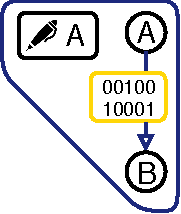
\includegraphics[width=.65\linewidth]{assets/tutorial_1}
%		\caption{To record an interaction between $ A $ and $ B $, $ A $ creates and sign a proposing micro-record (also called a \emph{proposal}).}
%		\label{fig:trustchain_tutorial_1}
%	\end{subfigure}%
%	\begin{subfigure}[t]{.33\textwidth}
%		\centering
%		\captionsetup{width=.89\linewidth}
%		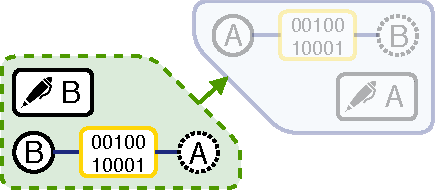
\includegraphics[width=.85\linewidth]{assets/tutorial_2}
%		\caption{Next, $ B $ confirms $ A $'s proposal by creating a confirming micro-record (also called a \emph{confirmation}), that points to it.}
%		\label{fig:trustchain_tutorial_2}
%	\end{subfigure}%
%	\begin{subfigure}[t]{.33\textwidth}
%		\centering
%		\captionsetup{width=.93\linewidth}
%		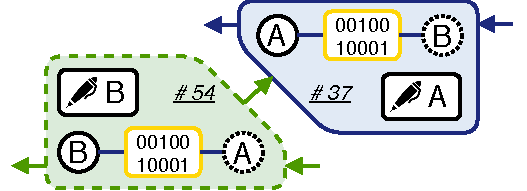
\includegraphics[width=.98\linewidth]{assets/tutorial_3}
%		\caption{To ensure tamper-proofness, we organize micro-records in personal ledgers and reference prior micro-records in a ledger.}
%		\label{fig:trustchain_tutorial_3}
%	\end{subfigure}
%	\caption{Storing an interaction between users $ A $ and $ B $ in \TrustChain{} using two micro-records, one proposal and one confirmation. Solid and dotted circular elements indicate the identity of the micro-record creator, respectively, the micro-record counterparty.}
%	\label{fig:trustchain_tutorial}
%\end{figure*}

\section{Accounting Work with \TrustChain{}}
\label{sec:micro_accounting}
The design of our universal accounting mechanism, named \emph{\TrustChain{}}, is inspired by the tamper-evident properties of blockchain but does not require peers to reach consensus on a coherent history of records.
Instead, \TrustChain{} optimistically detects the illegitimate modification of records while keeping the computational overhead and bandwidth requirements low.
Decentralized applications can account the work performed by peers within tamper-evident \emph{records}.
A record describes some work performed by one peer for another peer.
Each peer organizes their records in a \emph{personal ledger}.
Records point to prior records in the same personal ledger and also point to records in the personal ledger of others.
The latter pointer captures an agreement between two peers.
Peers continuously exchange records with other random peers and request records in the personal ledgers of others.
By validating the consistency of incoming records against known ones, a peer can irrefutably prove fraud attempts to other peers.

We further elaborate on the design of \TrustChain{}.
We first outline the network and threat model.
We then describe the \TrustChain{} data structure and show how \TrustChain{} accounts the work in decentralized applications.

\subsection{Network Model}
\label{sec:network_model}
The \TrustChain{} mechanism is built on a peer-to-peer network.
We assume an unstructured network structure.
Unstructured networks are relatively straightforward to maintain and are highly resilient against churn.
We assume that the used networking library handles network bootstrapping and peer discovery.
We also assume that the communication channels between peers are unreliable and unordered (e.g., by using the UDP communication model).
The arrival time of messages is not upper-bounded, and outbound messages can fail to arrive at their intended destination.
Each peer has a cryptographic key pair, consisting of a public and private key.
The public key acts as a unique identifier of the peer in the network, whereas the private key is used to sign records and outgoing network messages.
We consider attacks targeted at the network layer, e.g., the Eclipse Attack, outside the scope of this work.

A significant threat in Internet-deployed applications is the Sybil Attack, where an adversary operates multiple identities to subvert the network~\cite{douceur2002sybil}.
The Sybil Attack frequently occurs in open Internet communities, where the cost of creating a new digital identity is often negligible.
Although the \TrustChain{} mechanism does not include defences against Sybil identities, we argue that this threat can be mitigated with well-established techniques that complement \TrustChain{} in a deployment setting.
A basic defence mechanism is to have peers solve a computational puzzle when they wish to join the network~\cite{li2012sybilcontrol}.
In addition, using a Sybil-resistant reputation mechanism that processes \TrustChain{} records can effectively mitigate the effect of Sybil identities on computed trust scores~\cite{delaviz2012sybilres,yu2008sybillimit}.
We also consider self-sovereign identities as a promising solution that can bolster decentralized networks with long-term identities~\cite{stokkink2018deployment}.

We leave defences against misreporting, the accounting of work that has not occurred in the application, to other layers in the application stack.
This attack is closely related to the Sybil Attack since Sybil identities are likely to create fake interactions amongst them~\cite{stannat2021sybil}.
Misreporting is challenging to address in a generic manner since there is not always a straightforward method to assess if some accounted work is legitimate.
Some protocols use cryptographic techniques to prove the accuracy of performed work, for example, Proof-of-Storage and Proof-of-Bandwidth~\cite{benet2018filecoin,ghosh2014torpath}.
These proofs, however, cannot easily be used across different application domains.

\subsection{Threat Model}
\label{sec:threat_model}
Our threat model orients around malicious peers that attack the integrity of the \TrustChain{} data structure.
This attack proceeds through the strategic modification of \TrustChain{} records.
For example, a peer can inflate the amount of work it has performed by modifying one of the records in its personal ledger.
We refer to the illegitimate modification of \TrustChain{} records as \emph{fraud}.
Even though this definition may seem limited, we argue that this kind of fraud is a fundamental threat to the \TrustChain{} data structure.
In particular, our definition of fraud also entails a more advanced form of record manipulations where peers collude to erase a particular interaction from history.\footnote{Peers might refrain from overriding or erasing their records during or after a collusion attempt. We do not consider this as fraud since adversaries do not exploit the ConTrib data structure. Since all records associated with the collusion attempt are accounted, decentralized applications might employ additional logic to analyse created records and attempt to detect possible collusion attempts, e.g., with correlation analysis~\cite{liu2008detection}.}
In a reputation system, for example, this would happen when a well-trusted peer temporarily boosts the reputation of another peer by accounting some work and then attempts to hide the existence of this interaction later.
Reverting this interaction requires both counterparties to either override or remove the associated records, which we consider as fraud.
We note that a particular fraud instance in our system involves at most two guilty peers.
As we discussed in Section~\ref{sec:problem_description}, we require that fraud is detected.
We assume that the computing power of adversaries is bounded and that cryptographic primitives are secure.

% Hiding?

%A particular treat is when peers collude in order to record false information, e.g., a bandwidth upload that has not actually occurred within the system.
%It is non-trivial to verify whether the interaction has actually occurred in the system and therefore, we consider this attack outside our scope.
%Addressing this attack likely requires a mechanism that leverages application-specific properties.
%For example, TorPath builds a proof-of-bandwidth that proves that some bandwidth has been transferred through a circuit~\cite{ghosh2014torpath}.
%Creators of fake information should be given a lower trust score by the reputation mechanism, as illustrated in Figure~\ref{fig:trust_cycle}.

%Users store dual-signed agreements of their interactions using \TrustChain{} in \emph{micro-records}.

%\begin{table}
%\begin{center}
%	\begin{tabular}{ | p{1cm} | p{6.5cm} | }
%		\hline
%		\textbf{Field} &\textbf{Description} \\
%		\hline
%		$ i $ & The index of the micro-record in the personal ledger of $ a $. \\
%		$ a_{pk} $ & The public key of $ a $. \\
%		$ b_{pk} $ & The public key of $ b $. \\
%		$ t $ & The type of the micro-record. \\
%		$ p $ & The payload of the micro-record. \\ 
%		$ s_{a,i} $ & A digital signature by $ a $ over the micro-record. \\ 
%		$ h_{a,i-1} $ & The hash of the previous micro-record in the personal ledger of $ A $. \\ \hline
%		$ l $ & The index of the referenced proposal. \\ 
%		$ h_{b,l} $ & The hash of a referenced proposal. \\
%		\hline
%	\end{tabular}
%\end{center}
%\caption{The fields in a micro-record created by user $ a $, capturing an interaction with user $ b $. A proposal does not contain the last two fields ($ l $ and $ h_{b,l} $).}
%\label{tab:micro_record}
%\end{table}

\begin{figure}[t]
	\centering
	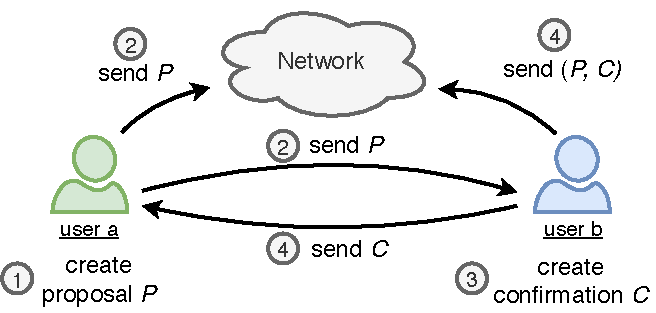
\includegraphics[width=.75\linewidth]{trustchain/assets/interaction}
	\caption{The process of recording work between peers $ a $ and $ b $ within two records: a proposal $ P $ and a confirmation $ C $.}
	\label{fig:interaction}
\end{figure}

\subsection{Recording Interactions}
\label{sec:recording_interactions}
Some work that involves peers $ a $ and $ b $ is recorded using two records: one \emph{proposal} created by $ a $ and one \emph{confirmation} created by $ b $.
W.l.o.g., we assume that the accounted work is performed by peer $ a $ for peer $ b $.
The process of accounting this work is visualized in Figure~\ref{fig:interaction}.
First, $ a $ creates a proposal record, which we refer to as $ P $ (step \circled{1}).
Proposal $ P $, created by peer $ a $, is a tuple with the following four attributes:
\begin{align*}
	P = (\texttt{pubKey}, \texttt{pubKeyOther}, \texttt{payload}, \texttt{sig})
\end{align*}
$ P $ contains the public key of peers $ a $ and $ b $ (\texttt{pubKey} and \texttt{pubKeyOther}, respectively), an application-specific payload (\texttt{payload}), and a digital signature (\texttt{sig}) created by $ a $ of the record in binary form.
The \texttt{payload} attribute is an arbitrary blob of data and is provided by the connected application.
To increase the resilience against manipulation, we extend records with additional fields in the next section.
After peer $ a $ has included all described attributes in the proposal, it persists the record to its database, sends the proposal to $ b $, and disseminated the proposal to $ f $ random peers in the network (step \circled{2}).
We refer to $ f $ as the \emph{fanout} value.

When peer $ b $ receives the proposal $ P $, $ b $ verifies its validity.
It is during this step that fraud is detected.
The validation logic of incoming records is elaborately discussed in Section~\ref{sec:detecting_fraud}.
If the incoming proposal $ P $ is deemed valid, the connected application determines if the payload in $ P $ truthfully describes the performed work.
If $ P $ considered invalid, $ b $ ignores the incoming proposal and takes no further action.
Otherwise, $ b $ creates a confirming record that confirms $ P $ (step \circled{3}).
This confirmation, denoted by $ C $, contains the same attributes as the proposal $ P $ and also includes the hash of $ P $.
Confirmation $ C $, created by peer $ b $ is a tuple with the following five attributes:
\begin{align*}
	C = (\texttt{pubKey}, \texttt{pubKeyOther}, \texttt{payload}, \texttt{proposalHash}, \texttt{sig})
\end{align*}

The value of \texttt{proposalHash} is computed by $ H(P) $, where $ H(\cdot) $ is a secure hash function.
We call the \texttt{proposalHash} attribute in $ C $ the \emph{confirmation pointer}.
After the creation of $ C $, peer $ b $ persists the confirmation to its database, sends it to $ a $, and disseminates both $ P $ and $ C $ to $ f $ random peers (step \circled{4}).
Upon the reception of $ C $, peer $ a $ validates the $ C $ and persists the confirmation if it is valid.
Both parties are now in possession of proposal $ P $ and confirmation $ C $ that together prove an agreement on work between these parties.
The process of accounting work is lightweight since it requires minimal computational power and data exchange. 
Also, peers can engage in the recording of multiple interactions simultaneously.

A potential risk is that $ b $ refuses to confirm $ P $, even though the incoming proposal is valid and contains the correct work details.
This could, for example, occur when confirming $ P $ negatively impacts $ b $'s social standing.
This leaves $ a $ with an unconfirmed proposal, which alone is not sufficient evidence to convince other peers of the performed work by $ a $ for $ b $.
When $ b $ refuses to sign an incoming proposal, $ a $ will add $ b $ to the local blacklist managed by applications, refusing to perform work for $ b $ until $ b $ has confirmed $ P $.
The losses for $ a $ depend on the magnitude of the (unconfirmed) work performed for $ b $.
To minimize these losses, we suggest that decentralized applications record small units of works using \TrustChain{}.
For example, a file-sharing application can choose to account unconfirmed work when it reaches a threshold, e.g., 10 MB of traffic exchanged.
Depending on the granularity of accounting, this approach can significantly reduce the impact of peers refusing to acknowledge the contributions of their counterparties.

\subsection{Improving Resilience by Linking Records}
To prevent the modification of created records, we enforce each peer in \TrustChain{} to link their records together in a \emph{personal ledger}, incrementally ordered by creation time.
Linking records will also make it harder for malicious peers to hide specific records.
We make the following four modifications to records:

\begin{enumerate}
	\item First, we include a sequence number $ s \in \mathbb{Z} $ in each record that is incremented by one when a new record is added to one's personal ledger.
	The sequence number of the first record in the personal ledger is 1.
	\item Second, each record now includes the hash of the prior record in the personal ledger of the creator.
	This modification makes the \TrustChain{} data structure comparable to a hash chain, e.g., as used by blockchain applications.
	The modification of a particular record now changes the hash of subsequent records, a feature that enables us to detect illegitimate changes to stored records (also see Section~\ref{sec:detecting_fraud}).
	The previous hash of the first record in a personal ledger is empty and referred to as $ \bot $.
	\item Third, we extend the confirmation pointer with the sequence number of the proposal record that it confirms.
	\item Forth, we include at most $ b $ additional hashes in each record of distinct, prior records in the same personal ledger.
	We indicate the set with these hashes with $ S $ and call these hashes \emph{back-pointers}.
	As we will further show in Section~\ref{sec:detecting_fraud}, the inclusion of these back-pointers significantly speeds up the detection of fraud.
	The required back-pointers in some record $ R $ are deterministically given by a pseudo-random function $ \sigma $ that takes the public key of the record creator and the sequence number of $ R $ as input.
	$ \sigma $ returns a set with at most $ b $ prior records which hashes should be included in $ R $.
	All peers must use the same version of $ \sigma $, which we achieve by bundling its implementation in the \TrustChain{} software.
\end{enumerate}

The above modifications change the attributes of proposal and confirmation records.
We re-define a proposal $ P $, created by peer $ a $ and with counterparty $ b $, as follows:
\begin{align*}
	P = (\texttt{pubKey}, \texttt{pubKeyOther}, \texttt{payload}, \texttt{sig}, \textcolor{ao}{\texttt{seqNum}}, \textcolor{ao}{\texttt{prevHash}}, \textcolor{ao}{\texttt{backPointers}})
\end{align*}
The variables coloured green are new compared to our previous definition of $ P $.
\texttt{seqNum} refers to the sequence number of $ P $, \texttt{prevHash} indicates the hash of the previous record, and \texttt{backPointers} is the set with back-pointers (where $ |S| \leq b $).
We re-define a confirmation $ C $, created by peer $ b $, as follows:
\begin{align*}
	C = (\texttt{pubKey}, \texttt{pubKeyOther}, \texttt{payload}, \textcolor{ao}{\texttt{linkInfo}}, \texttt{sig},
	\textcolor{ao}{\texttt{seqNum}}, \textcolor{ao}{\texttt{prevHash}}, \textcolor{ao}{\texttt{backPointers}})
\end{align*}

We extend confirmations with the same attributes as a proposal but replace the \texttt{proposalHash} attribute with \texttt{linkInfo}.
This is in accordance with our third modification.
\texttt{linkInfo} is now defined as a tuple with the hash and sequence number of the referred proposal record:
\begin{align*}
	C.\texttt{linkInfo} = (\texttt{hash}, \texttt{seqNum})
\end{align*}

Creating records yields the graph structure, as shown in Figure \ref{fig:fullchain}.
Figure \ref{fig:fullchain} shows a part of the \TrustChain{} graph with six records, created by three distinct peers ($ a $, $ b $ and $ c $).
Same-coloured records are part of a single personal ledger, and arrows represent hash pointers to other records.
Proposals have a solid border whereas confirmations have a dashed border.
Note how the record in $ a $'s personal ledger with sequence number 55 is unconfirmed.
For presentation clarity, we only show the pointer to the prior record in one's personal ledger and omit additional back-pointers from the figure.

\begin{figure}[t]
	\centering
	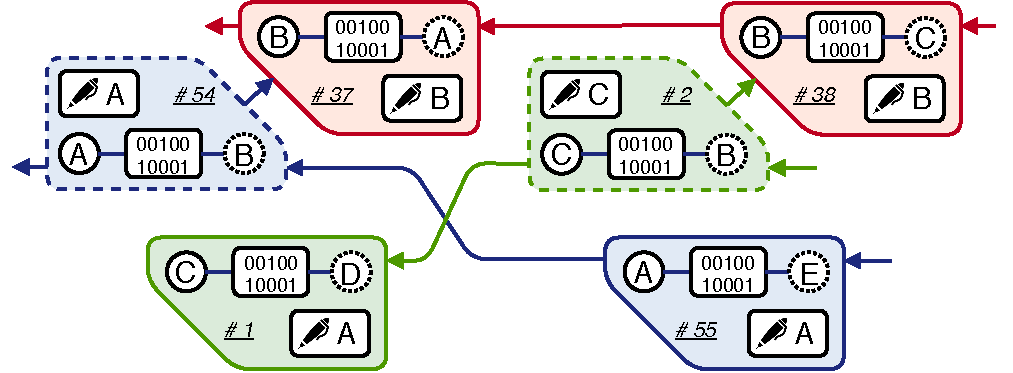
\includegraphics[width=.9\linewidth]{trustchain/assets/fullchain}
	\caption{A part of the \TrustChain{} DAG, involving five peers and six records: four proposals (solid borders) and two confirmations (dashed borders). The proposal created by user $ a $ with sequence number 55 is unconfirmed.}
	\label{fig:fullchain}
\end{figure}

\TrustChain{} publicly accounts work in interlinked personal ledgers.
Since all performed work is publicly stored and accessible, other users might acquire and analyse \TrustChain{} records to reveal potentially sensitive information, e.g., the time at which a particular user is online or the interaction patterns between users.
To reduce this threat, we outline two techniques that applications can use to enhance privacy.
First, applications can account performed and consumed work in \emph{batches}.
For example, an application can record all outstanding contributions and consumptions every hour, therefore hiding granular work statistics.
Second, an application can add some noise to the amount of work being accounted (\emph{fuzzy accounting}).
This technique effectively reduces linkability, e.g., when accounting traffic that is being relayed through multiple hops.
We believe that the combined power of these two techniques provides sufficient privacy guarantees for most decentralized applications.
A more advanced approach, used by the Monero cryptocurrency, leverages ring signatures and zero-knowledge proofs to hide the amounts of work performed~\cite{bunz2018bulletproofs,poelstra2018confidential}.
This approach would, however, require fundamental changes to \TrustChain{} and we leave this enhancement for further work.

\section{Detecting Fraud}
\label{sec:detecting_fraud}
We require that \TrustChain{} detects illegitimate tampering of the records in a personal ledger.
\TrustChain{} is built around fraud \emph{detection} instead of \emph{prevention}.
We argue this is a reasonable assumption for two reasons.
First, decentralized applications often do not require the prevention of fraud~\cite{krishnan2002virtual}.
We argue that fraud prevention is disproportional in the context of work accounting.
Second, preventing fraud is often a resource-intensive process that requires peers to reach a consensus on all created records, e.g., by using classical BFT algorithms or Proof-of-Work~\cite{vukolic2015quest}.
The requirement to reach consensus would severely limit the scalability of \TrustChain{}.

Fraud in \TrustChain{} occurs when a peer illegitimately modifies one of the records in their personal ledger.
This fraud, for example, happens when an adversary attempts to hide a specific record in the personal ledger by replacing it with another one.
This action would result in pairs of records with the same sequence number and the same creator, but with a different hash.
This violates the integrity of the \TrustChain{} data structure.
A key objective of \TrustChain{} is to detect such conflicting records quickly.

%According to our threat model, manipulation in \TrustChain{} involves an adversary maintaining two different personal ledgers, possibly with a common prefix.
%In related literature, this is often referred to as double-spending or chain forking.

%To incentivize users to participate in the exploration of the \TrustChain{} DAG, we propose that collected fraud proofs can be given to resource providers to gain preferential treatment.\todo{elaborate}
%For example, a user $ A $ can modify, reorder or remove micro-records in their personal ledger, and recompute the hash pointers to restore validity.
%However, this basic manipulation can be proven by interaction partners of $ A $ by having them broadcasting the original and manipulated micro-records created by $ A $ with the same sequence number.

%To prove this fraud to others, a user can broadcast the original and manipulated micro-records.

\begin{figure*}[t!]
	\centering
	\begin{subfigure}[t]{.5\textwidth}
		\centering
		\captionsetup{width=.9\linewidth}
		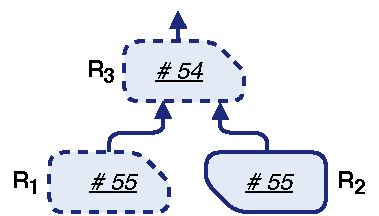
\includegraphics[width=.75\linewidth]{trustchain/assets/fraud_scenario_1}
		\caption{\emph{Scenario I}: Records $ R_1 $ and $ R_2 $ have the same sequence number but a different hash. The pair $ (R_1, R_2) $ is irrefutable proof that peer $ a $ has forked its personal ledger.}
		\label{fig:fraud_scenario_1}
	\end{subfigure}%
	\begin{subfigure}[t]{.5\textwidth}
		\centering
		\captionsetup{width=.89\linewidth}
		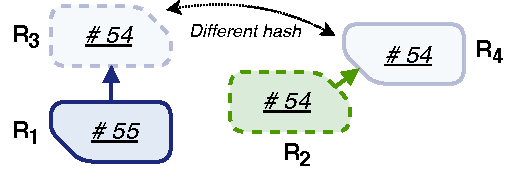
\includegraphics[width=.75\linewidth]{trustchain/assets/fraud_scenario_2}
		\caption{\emph{Scenario II}: Records $ R_3 $ and $ R_4 $ both contain a back-pointer to the record with sequence number 54 but their hashes differ. The pair $ (R_3, R_4) $ is irrefutable proof that peer $ a $ has forked its personal ledger.}
		\label{fig:fraud_scenario_2}\vspace{0.9cm}
	\end{subfigure}
	\begin{subfigure}[t]{.5\textwidth}
		\centering
		\captionsetup{width=.89\linewidth}
		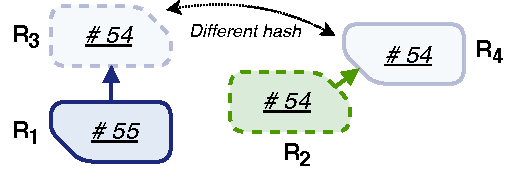
\includegraphics[width=\linewidth]{trustchain/assets/fraud_scenario_3}
		\caption{\emph{Scenario III}: Records $ R_1 $ and $ R_2 $ contain a differing hash of $ a $'s record with sequence number 54. This reveals an inconsistency.}
		\label{fig:fraud_scenario_3}\vspace{0.9cm}
	\end{subfigure}
	\begin{subfigure}[t]{.6\textwidth}
		\centering
		\captionsetup{width=.89\linewidth}
		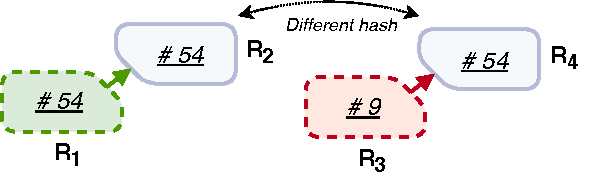
\includegraphics[width=.98\linewidth]{trustchain/assets/fraud_scenario_4}
		\caption{\emph{Scenario IV}: Records $ R_1 $ and $ R_3 $ both confirm $ a $'s record with sequence number 54, but they contain a different hash. This reveals an inconsistency.}
		\label{fig:fraud_scenario_4}
	\end{subfigure}
	\caption{Four scenarios that allows a peer to either expose fraud (forking of a personal ledger), or to detect an inconsistency (without assigning blame). The colour of each record indicates the identity of its creator (blue for $ a $, green for $ b $ and red for $ c $). Solid and dashed records indicate proposals, respectively confirmations. Opaque records are not in possession by the peer.}
	\label{fig:fraud_scenarios}
\end{figure*}

\subsection{Detecting Forks}
\label{sec:detecting_forks}
Fraud in \TrustChain{} is detected by sharing newly created records with other peers, and by requesting random records in the personal ledgers of others.
Each peer assesses the consistency of incoming records with the ones in its local database.
This simple approach allows for quick detection of fraud through the collective effort of peers.
In Figure~\ref{fig:fraud_scenarios}, we visualize four identified scenarios in which we can either expose an adversarial peer (scenario I and II) or detect an inconsistency without assigning blame (scenario III and IV).
Each scenario shows the situation from a single peer's perspective and highlights records that a peer has in its local database, or does not have.
Records not in the possession by a peer are faded.
Records with the same colour are created by the same peer.
We discuss each scenario and elaborate on how they either lead to fraud exposure or the detection of an inconsistency.

\begin{itemize}
	\item \textbf{Scenario I}. 
	The first scenario, visualized in Figure~\ref{fig:fraud_scenario_1}, describes a situation where a peer can directly expose a fork in the personal ledger of peer $ a $.
	The personal ledger of peer $ a $ has been forked since records $ R_1 $ and $ R_2 $ have the same sequence number but a different hash.
	As soon as another peer, say $ b $, receives $ R_1 $ while already having $ R_2 $, or receives $ R_2 $ while already having $ R_1 $, the pair $ (R_1, R_2) $ is sufficient evidence to expose the fraud by $ a $.
	The digital signature by $ a $ in the records prove that $ a $ deliberately created both records.
	Note that $ b $ does not need to have $ R_3 $ to detect nor to prove this fraud.
	We call the pair $ (R_1, R_2) $ a \emph{fraud proof}.
	Fraud proofs are by default shared with other peers in the network through a \texttt{FraudProof} message.
	\item \textbf{Scenario II}. The second scenario describes the situation where one can prove fraud by detecting inconsistencies in the included back-pointers of records.
	Figure~\ref{fig:fraud_scenario_2} shows four records created by peer $ a $.
	Records $ R_3 $ and $ R_4 $ contain the hash of the record with sequence number 54 in the back-pointer set; however, these back-pointers describe the same record with a different hash.
	The pair $ (R_3, R_4) $ is irrefutable proof that peer $ a $ has committed fraud and can be used to construct a fraud proof.
	\item \textbf{Scenario III}.
	Figure~\ref{fig:fraud_scenario_3} shows a third scenario where a peer receives proposal $ R_1 $ and already has confirmation $ R_2 $, or receives confirmation $ R_2 $ while already having proposal $ R_1 $.
	The peer does not have records $ R_3 $ and $ R_4 $.
	The hash of record $ R_3 $ in $ R_1 $ differs from the hash in the confirmation pointer in $ R_2 $.
	This situation reveals an inconsistency that is either introduced by peer $ a $ forking its personal ledger at height 54, or by $ b $ having included a wrong hash in $ R_2 $.
	To assign blame, the peer that is validating the incoming record requires either $ R_3 $ or $ R_4 $.
	A peer that encounters this situation sends the pair ($ R_1 $, $ R_2 $) within a \texttt{Inconsistency} message to other random peers, hoping that others will be able to expose the malicious peer.
	\item \textbf{Scenario IV.}
	Figure~\ref{fig:fraud_scenario_4} highlights the fourth scenario where a peer either receives confirmation $ R_1 $ while already having confirmation $ R_3 $, or vice versa.
	Both confirmations point to a record with the same public key and sequence number, but the hash of this record differs.
	This situation either indicates a fork of the personal ledger of $ a $, or it can be the result of an invalid pointer in one of the confirmations.
	Similar to scenario III, the validating peer sends the pair ($ R_1 $, $ R_3 $) within a \texttt{Inconsistency} message to other, random peers.
\end{itemize}

%The other two scenarios, displayed in Figure~\ref{fig:fraud_scenario_2} and Figure~\ref{fig:fraud_scenario_3}, enables the detection of an inconsistency but one cannot assign blame without more context.

%A more advanced manipulation is \emph{forking}, where a user creates two micro-records with the %same sequence number but with different counterparties.
%The goal of this fraud is to hide a specific micro-record from ones personal ledger, e.g., records that indicate some resource consumptions.
%This is similar to the double-spend attack in blockchain ledgers like Bitcoin~\cite{grunspan2018double}.
%Only when a user discovers both conflicting micro-records, this manipulation can be proven.
%In Section~\ref{sec:fraud_detection_experiment} we demonstrate that this fraud can be detected within seconds.
%To prove this fraud, the transaction counterparty reveals both the correct block and the invalid block created by $ A $.

\begin{algorithm}[!t]
	\caption{The validation of the fields in record $ R $.}
	\label{alg:record_data_validation}
	\begin{algorithmic}[1]
		\Procedure{validateFields}{$ R $}  \Comment{Step 1}
		\State $ valid \leftarrow $ true
		\If{$ R.seqNum < 1 $}
		\State $ valid \leftarrow $ false
		\EndIf
		
		\If{\textsc{isConfirmation($ R $)} \textbf{and} $ R.linkInfo.seqNum < 1 $}
		\State $ valid \leftarrow $ false
		\EndIf
		
		\If{\textbf{not} \textsc{publicKeyIsValid}($ R.pubKey $)}
		\State $ valid \leftarrow $ false
		\EndIf
		
		\If{\textbf{not} \textsc{signatureIsValid}($ R.pubKey $, $ R.sig $)}
		\State $ valid \leftarrow $ false
		\EndIf
		
		\If{\textbf{not} \textsc{publicKeyIsValid}($ R.pubKeyOther $)}
		\State $ valid \leftarrow $ false
		\EndIf
		
		\If{$ R.seqNum = 1 $ \textbf{and} $ R.prevHash \not= \bot $}
		\State $ valid \leftarrow $ false
		\EndIf
		
		\State \Return valid
		\EndProcedure
		
	\end{algorithmic}
\end{algorithm}

\subsection{Record Validation Logic}
\label{sec:validation_logic}
Based on the four identified scenarios, we design and describe the validation logic of an incoming record $ R $.
Each peer keeps track of known hashes in a dictionary named \texttt{knownHashes}.
This dictionary is indexed with a tuple, containing the public key and sequence number of a record.
The value of dictionary entries is the hash of the record being queried.
%To simplify the validation logic, proposals and confirmations have the same fields.
%The confirmation pointer is implemented with three fields: \textsc{linkPublicKey}, \textsc{linkSeqNum} and \textsc{linkHash}.
%In a proposal, these fields are set to \textsc{null}.
%Each user maintains a dictionary \textsc{hashes} with known hashes.
The validation logic of incoming records consists of the following five steps:

\begin{algorithm}[t]
	\caption{The validation of an incoming record against a linked record.}
	\label{alg:record_validation_step3}
	\begin{algorithmic}[1]
		\Procedure{validateLink}{R}  \Comment{Step 3}
		\State $ linked \leftarrow db $.\textsc{getLinked(R)}
		\If{$ linked = \bot $}
		\State \Return true
		\EndIf
		\State
		\State $ proposal \leftarrow linked $ \textbf{if} \textsc{isConfirmation(R)} \textbf{else} $ R $
		\State $ confirmation \leftarrow linked $ \textbf{if} \textsc{isConfirmation($ linked $)} \textbf{else} $ R $
		\State
		\If{$ confirmation.pubKeyOther \not= proposal.pubKey $}
		\State \Return false
		\EndIf
		\If{$ confirmation.linkInfo.seqNum \not= proposal.seqNum $}
		\State \Return false
		\EndIf
		\If{$ confirmation.linkInfo.hash \not= proposal.hash $}
		\State \Return false
		\EndIf
		\State $ linkLinked \leftarrow $ db.\textsc{getLinked(}$ linked $\textsc{)}
		\If{$ linkLinked \not= \bot $ \textbf{or} $ link\_linked \not= R $}
		\State \Return false
		\EndIf
		\State \Return true
		\EndProcedure
	\end{algorithmic}
\end{algorithm}

\textbf{Step 1.}
We first verify the validity of the fields in incoming record $ R $.
This step is performed by the \textsc{validateFields} procedure, which returns a boolean value indicating whether the fields in the record are valid or not.
A pseudocode description of this procedure is given in Listing~\ref{alg:record_data_validation}.
This step validates the sequence number (line 3), the included public keys (line 7 and 11), and the digital signature (line 9).
If the incoming record is a confirmation, it also verifies that the sequence number in the \texttt{linkInfo} attribute is within a valid range (line 5).
It also checks whether the hash of the prior record is sane when the record is the first in ones personal ledger (line 13).
This step does not compare the validity of $ R $ within the context of other records.
Any error in the included fields of $ R $ is computationally efficient to detect and likely originates from a software bug.

\textbf{Step 2.}
Next, we query the database for a record with the same public key and sequence number as the incoming record $ R $.
If such a record $ R' $ is in the database, we check the equality of $ R $ and $ R' $ by performing a comparison between their included fields.
If $ R \not= R' $, we have detected a fork in the personal ledger of the creator behind $ R $.
We then share the fraud proof $ (R, R') $ with other peers in the network.
During this step, we detect the fraud described by scenario I in Section~\ref{sec:detecting_forks}.

\textbf{Step 3.}
Then, we verify if the hash pointers in the incoming record are consistent with known ones.
This is performed by the \textsc{validateHashes} procedure which pseudocode description is given in Listing~\ref{alg:record_validation_step4}.
This procedure first checks whether the \texttt{prevHash} attribute in $ R $ is consistent with the information in the \texttt{knownHashes} dictionary (line 3).
We then iterate over all included back-pointers and verify the consistency of these hashes with the entries in the \texttt{knownHashes} dictionary (line 6-10).
We can detect the inconsistency described by scenario II during this step.

\textbf{Step 4.}
Next, we compare incoming record $ R $ with a link record, if such a record is available in the database.
When $ R $ is a proposal, we get the corresponding confirmation from the database, and if $ R $ is a confirmation, we get the corresponding proposal.
This step is performed by the the \textsc{validateLink} procedure which pseudocode description is given in Listing~\ref{alg:record_validation_step3}.
We first get the linked record from the database (line 2) and only continue with this validation step if we have this record in the database.
We check whether the public keys included in the proposal and confirmation are consistent (line 9), and verify the consistency of the \texttt{linkInfo} attributes in the confirmation (line 11-14).
We detect the inconsistency described by scenario III during this step (line 15-17).

\textbf{Step 5.}
Finally, we verify the validity of the included payload, which is an application-dependent validation procedure.
As we will further outline in Section~\ref{sec:system_architecture}, decentralized applications using \TrustChain{} should implement a \emph{validation} policy that denotes whether the payload of an incoming record is valid in the context of the connected application.

If any of the above steps fail, the record is considered invalid.

\begin{algorithm}[t]
	\caption{The consistency validation of hashes in an incoming record against known ones.}
	\label{alg:record_validation_step4}
	\begin{algorithmic}[1]
		
		\Procedure{validateHashes}{R}  \Comment{Step 4}
		\State $ hash \leftarrow knownHashes[(R.pubKey, R.seqNum - 1)] $
		\If{$ hash \not= \bot $ \textbf{and} $ hash \not= R.prevHash $}
		\State \Return false
		\EndIf
		\State
		\For{$ seqNum, hash $ \textbf{in} $ R.backPointers $}
		\State $ known \leftarrow knownHashes[(R.pubKey, seqNum)] $
		\If{$ known \not= \bot $ \textbf{and} $ hash \not= known $}
		\State \Return false
		\EndIf
		\EndFor
		\State \Return true
		\EndProcedure
		
	\end{algorithmic}
\end{algorithm}

\subsection{Exchanging Records with Other Peers}
\label{sec:exchanging_records}
The detection of fraud in \TrustChain{} depends on peers exchanging records with each other.
A peer is motivated to share collected records with others since they might eventually reveal fraud conducted by one of their former counterparties.
So far, we have not discussed how records are disseminated.
Record dissemination is an essential process that affects the speed at which fraud can be detected.
For example, a slow record exchange strategy is likely to increase fraud detection times compared to more aggressive record dissemination.
We consider both \emph{push-based} and \emph{pull-based} exchange of records, which is explained next.

\textbf{Pull-based Record Exchange.}
Each peer by default requests (pulls) records from other random peers at a fixed rate by sending out \texttt{Request} messages.
Applications can choose to send out \texttt{Request} messages to specific peers to build profile information about that peer, e.g., to detect free-riders.
A \texttt{Request} message contains a list of sequence numbers that the recipient should send back.
When receiving a \texttt{Request} message, the recipient also includes linked proposal or confirmation records in the response.
When a peer $ a $ does not respond with records within a reasonable time, the requesting peer adds $ a $ to the local blacklist.

\textbf{Push-based Record Exchange.}
\TrustChain{} also supports push-based record exchange, where the creator of a record disseminates it to $ f $ random other peers (as also discussed in Section~\ref{sec:recording_interactions}).
This push-based exchange allows for quick detection of fraud since the probability of no user receiving two conflicting records goes to zero quickly, even when the network size increases~\cite{osipkov2007combating}.
Even if the malicious peer refrains from broadcasting a conflicting record, the counterparty is very likely to do so, assuming there is no collusion between interacting peers.
Immediate dissemination of created records in the network also increases record availability when the sending peer goes offline.

\begin{figure*}[t]
	\centering
	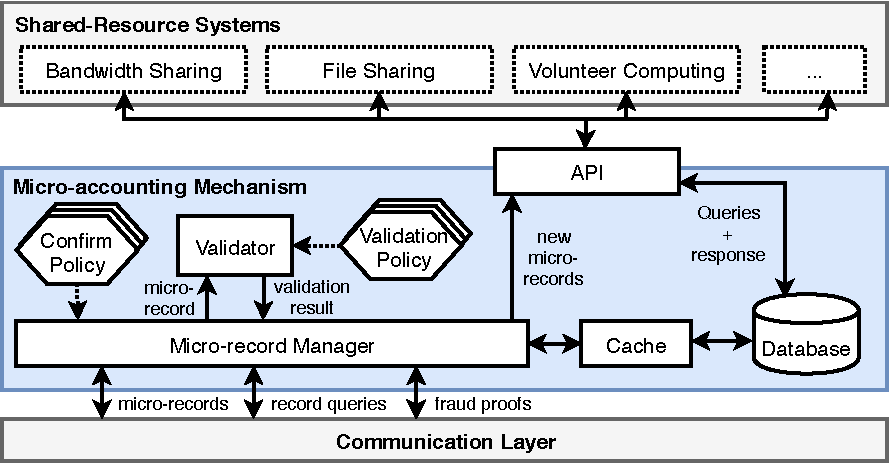
\includegraphics[width=\linewidth]{trustchain/assets/system_architecture}
	\caption{The system architecture of \TrustChain{}.}
	\label{fig:system_architecture}
\end{figure*}

\subsection{Limitations}
%In Section~\ref{sec:micro_accounting} and~\ref{sec:detecting_fraud}, we have described how \TrustChain{} records are created and how fraud is detected.
Even though our simple algorithm can detect the modification of records, the probabilistic nature of our algorithm can render \TrustChain{} unsuitable for deployment in specific application domains.
Since fraud detection is a probabilistic approach, some fraud instances can take relatively long to be uncovered (e.g., several minutes).
We also encountered this behaviour during our experiments (see Section~\ref{sec:implementation_evaluation}).
At the same time, we argue that this is not an insurmountable problem in decentralized applications where performed work holds no or low monetary value.

Since our algorithm is based on fraud \emph{detection}, \TrustChain{} is not suitable for applications that require a high level of security, as is the case with decentralized financial applications.
We believe that blockchain technology provides more appropriate security guarantees for such application domains, at the cost of increased resource usage and lower scalability.

Finally, we note that \TrustChain{} is mainly built for the lightweight accounting of work in decentralized applications.
In its current state, \TrustChain{} cannot capture more complicated operations, e.g., executing arbitrary logic like smart contracts.
However, as demonstrated by recent research advancements, a lightweight accounting mechanism can be an enabling component to devise novel types of decentralized applications with dynamic risk guarantees~\cite{de2021xchange,de2019devid,de2018real}.

% Limitations:
% 1. optimistic detection of fraud -> not everything is detected
% 2. fraud detection is a probablistic process -> detection can take long, depending on several factors

\section{System Architecture}
\label{sec:system_architecture}
We devise a system architecture of our \TrustChain{} mechanism, see Figure~\ref{fig:system_architecture}).
The network layer is the lowest layer in our architecture and provides the primitives for decentralised communication and peer discovery.
This layer can be realised using existing frameworks to build peer-to-peer overlay networks, for example, libp2p.\footnote{See \url{https://libp2p.io}}

\textbf{Record Manager.}
The record manager interacts with the network layer to disseminate records and processes incoming ones.
It queues incoming records for validation and persists incoming fraud proofs to the database and connected application.
It also manages the confirmation of incoming and valid proposals targeted at that peer.
Applications using \TrustChain{} should provide a \emph{confirmation policy} that predicates whether an incoming proposal should be confirmed.

\textbf{Validator.}
The validator determines the validity of incoming records according to the algorithms described in Section~\ref{sec:validation_logic}.
Connection applications can provide a custom \emph{validation policy}.
If provided, this validation policy is invoked during step 5, when the application-specific payload in a record is validated.
The flexibility to provide custom validation and confirmation policies for incoming records makes \TrustChain{} universal and reusable across different application domains.

\textbf{Persistence.}
Records and fraud proofs are persisted in a database.
The \TrustChain{} system architecture provides an interface for the queries made to the database and supports different database architectures, e.g., structured or unstructured models.
Our system architecture includes a record \emph{cache}, which is an intermediary component that stores all records in the personal ledger of the operating peer in memory.
This cache allows \TrustChain{} to quickly respond to incoming record queries in the personal ledger of the operating peer.
This cache forwards queries to the database for the retrieval and storage of records and fraud proofs.

To contain the growth of the database and to keep the storage overhead manageable, an application can choose to periodically prune the \TrustChain{} database when a storage threshold is reached.
In our implementation, by default, we start pruning when at least one million records have been stored.
Applications may increase or decrease this number, depending on the storage capacities of participating peers and the deployment environment.
The default pruning strategy of \TrustChain{} continuously removes the record with the lowest database insertion timestamps until the database size has reached its storage threshold again.
The pruning of older records might cause some forks to go undetected since records are removed before a fraud proof can be constructed.
As we will show in Section~\ref{sec:fraud_detection_experiment}, most forks in \TrustChain{} are quickly detected, and there should be ample time to detect inconsistencies before relevant records are pruned.

\textbf{Fraud Management.}
When the validation algorithm exposes fraud, or when \TrustChain{} receives an incoming fraud proof, the connected applications are notified of the fraud and can punish the misbehaving peer accordingly.
For example, a fraud policy in a bandwidth sharing application could decide to not serve the fraudster for some time.
The decentralised application store the digital identities of fraudsters in a local blacklist.

\textbf{Interactions between \TrustChain{} and Applications.}
Decentralised applications interact with \TrustChain{} through an API.
This API allows connected applications to query the content of the database.
Furthermore, connected applications can subscribe to incoming records.
The record manager forwards new records to the API, which passes these records to subscribed applications.

\begin{table}[]
	\begin{center}
		\begin{tabular}{l l}
			\hline
			\textbf{Parameter} & \textbf{Default Value}  \\ \hline
			Peers ($ n $) & 1'000 \\
			Workload & 1 proposal per second per peer \\
			Record exchange strategy & \texttt{PULL+RAND+PUSH} \\
			Record fanout ($ f $) & 5 \\
			Record request batch size & 2 \\
			Record request interval & 0.5 seconds \\
			Packet Loss Rate & 0\% \\
			Individual forking probability & 10\% \\
			Back-pointers ($ b $) & 10 \\ \hline
		\end{tabular}
		\caption{The default parameters used during our evaluation.}
		\label{tab:experiment_parameters}
	\end{center}
\end{table}


\section{Implementation and Evaluation}
\label{sec:implementation_evaluation}
Within this section we systematically explore how \TrustChain{} behaves when modifying system parameters.
%In the next section we observe how the full implementation of \TrustChain{} behaves under real-world conditions and with real Internet users.
We implement \TrustChain{} in the Python 3 programming language.
We leverage the network library implemented by our group, and use the UDP protocol for network communication.\footnote{See \url{https://github.com/tribler/py-ipv8}}
Our implementation uses the \texttt{asyncio} framework for asynchronous event handling.
The implementation features both an in-memory storage for experimentation and a persistent (sqlite) database which can be used to persist records over different sessions.
The full implementation of \TrustChain{}, including unit tests and documentation, is published on GitHub.\footnote{See \url{https://github.com/tribler/py-ipv8/tree/master/ipv8/attestation/trustchain}}

\subsection{Experiment Setup}
We evaluate the impact of different parameters on the efficiency of fraud detection.
We do so by measuring the time between committing the fraud and its initial detection.
We substitute our networking layer with the SimPy discrete event simulator~\cite{matloff2008introduction}.
Each peer in the \TrustChain{} network knows the network address of 100 random other peers, resulting in an unstructured overlay topology.
Table~\ref{tab:experiment_parameters} lists the default parameters during our experiments.
To encourage reproducibility, we have open-sourced the \TrustChain{} simulator and all experiment scripts.\footnote{See \url{https://github.com/tribler/trustchain-simulator-pysim}}

\textbf{Workload and Attack Model.}
During our experiments, peers create records with other random peers.
Our default workload has each peer initiate one proposal per second with another random peer.
Note that the rate at which new records are created grows with the network size, which should capture the dynamics of real-world applications (when there are more peers, there is usually more work performed in the application).
We use a uniform transaction load to analyse the characteristics of \TrustChain{} under a predictable load.
Even though this transaction load is predictable, it resembles an application where work is periodically accounted.
We experiment with network sizes ranging from 1'000 to 10'000 online peers.
Though some deployed networks have many more peers (e.g., BitTorrent and Tor), our experimental results suggest that \TrustChain{} has no issues scaling beyond 10'000 peers.
In Section~\ref{subsec:realistic_workload}, we subject \TrustChain{} to a realistic workload, extracted from the interactions in a decentralized file-sharing application.

Each peer forks its personal ledger with a probability of 10\% by removing the last record in its personal ledger and re-using its sequence number to create a new record.
Each peer commits this fraud once.
A peer committing fraud will not broadcast the duplicate record when push-based record exchange is enabled.
In each experiment run, all peers start with an empty personal ledger, and interaction partners always confirm incoming proposals.
A peer that has exposed the fraud of another peer will refuse to confirm the proposals by that peer.
Each experiment run terminates either when all fraud attempts have been discovered or after ten minutes have elapsed.
We are interested in the detection time of fraud instances, which is the time period between committing the fraud and its first detection by a peer in the network.

\textbf{Record Exchange Strategies.}
We consider the following four strategies for exchanging records.
With the \texttt{PULL} strategy, each peer requests two contiguous records at a random height in the personal ledger of another random peer every half a second (the \emph{record request batch size} and \emph{record request interval} parameters in Table~\ref{tab:experiment_parameters}).
Under the \texttt{PULL+RAND} strategy, a peer also returns five random records in their database upon a query.
Including random records in responses enables the detection of fraud of offline peers.
The \texttt{PULL+PUSH} strategy also pushes new records to $ f $ random users upon creation, compared to the \texttt{PULL} strategy.
Finally, we consider the \texttt{PULL+RAND+PUSH} record exchange strategy, which is a combination of the above techniques.

\begin{figure*}[t]
	\centering
	\begin{subfigure}{.8\columnwidth}
		\centering
		
\includegraphics[width=.8\linewidth]{trustchain/assets/fraud_experiments_legend}
	\end{subfigure}
	\begin{subfigure}{.5\columnwidth}
		\centering
		\captionsetup{width=.9\linewidth}
		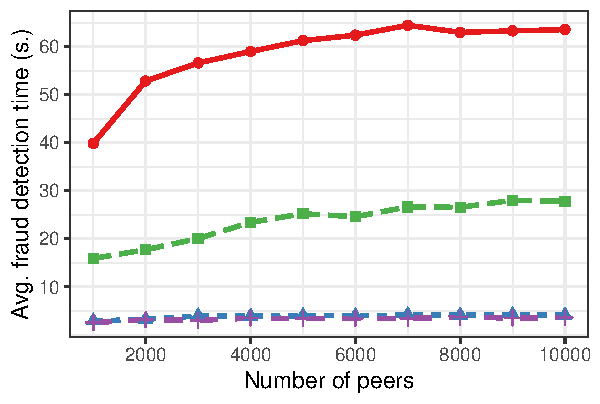
\includegraphics[width=\linewidth]{trustchain/assets/fraud_times_scalability}
		\caption{Average fraud detection times as the number of peers increases.}
		\label{fig:experiment_scalability_detection_times}
	\end{subfigure}%
	\begin{subfigure}{.5\columnwidth}
		\centering
		\captionsetup{width=.9\linewidth}
		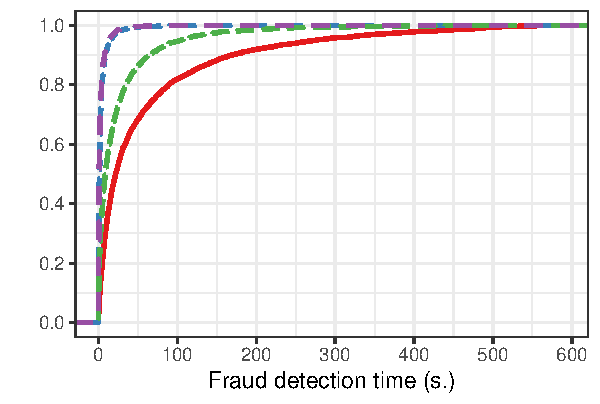
\includegraphics[width=\columnwidth]{trustchain/assets/fraud_times_scalability_5000_ecdf}
		\caption{The Empirical Cumulative Distribution Function (ECDF) for 5'000 peers.}
		\label{fig:experiment_scalability_ecdf_detection_times}
	\end{subfigure}
	\begin{subfigure}{.5\columnwidth}
		\centering
		\captionsetup{width=.9\linewidth}
		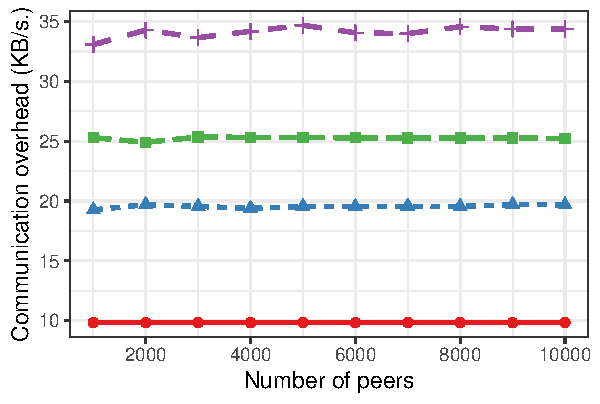
\includegraphics[width=\linewidth]{trustchain/assets/scalability_bandwidth_usage}
		\caption{Average network usage per peer as the number of peers increases.}
		\label{fig:experiment_scalability_bandwidth}
	\end{subfigure}%
	\begin{subfigure}{.5\columnwidth}
		\centering
		\captionsetup{width=.9\linewidth}
		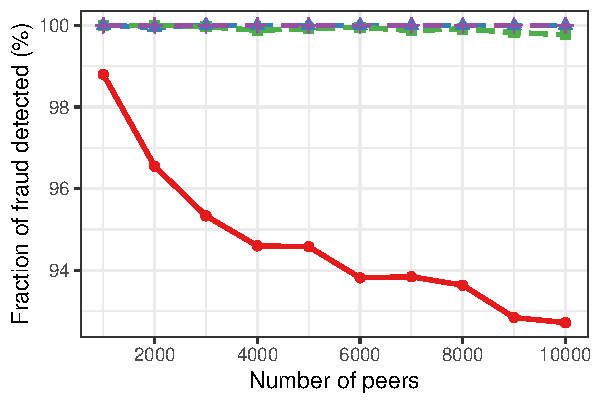
\includegraphics[width=\columnwidth]{trustchain/assets/scalability_num_detected}
		\caption{Fraction of fraud exposed after our experiment ends.}
		\label{fig:experiment_scalability_num_detected}
	\end{subfigure}
	\caption{The results of our scalability experiments, with up to 10'000 peers. We evaluate four record exchange strategies.}
	\label{fig:scalability_experiments}
\end{figure*}

\subsection{Scalability}
\label{sec:fraud_detection_experiment}
Our first experiment quantifies the scalability of \TrustChain{} when increasing the number of peers in the network, see Figure~\ref{fig:scalability_experiments}.
Figure~\ref{fig:experiment_scalability_detection_times} shows the effect of increasing the number of peers on the average time until fraud detection, for the four discussed record exchange strategies.
For all record exchange strategies, the average fraud detection time seems to increase when the network size grows.
For $ n = 10'000 $, the \texttt{PULL} strategy shows an average fraud detection time of 63.5 seconds, whereas this number decreases to 3.6 seconds under the \texttt{PULL+RAND+PUSH} strategy.
We notice that the \texttt{PULL+PUSH} and \texttt{PULL+RAND+PUSH} strategies show detection times under five seconds on average.
These low detection times demonstrates that disseminating a record just after its creation is a highly successful strategy.
Including random records in crawl responses also seems to decrease the average fraud detection times.
For $ n = 10'000 $, the average fraud detection time decreases from 63.5 seconds for the \texttt{PULL} strategy to 27.8 seconds for the \texttt{PULL+PUSH} strategy.

In Figure~\ref{fig:experiment_scalability_ecdf_detection_times}, we show the Empirical Cumulative Distribution Function (ECDF) of fraud detection times for $ n = 5'000 $.
We observe that it can take several minutes for some fraud attempts to be discovered, in particular for the \texttt{PULL} and \texttt{PULL+RAND} strategies.
This is not unexpected since fraud detection in \TrustChain{} is a highly probabilistic approach.
For the \texttt{PULL} strategy, we can detect 90\% of fraud attempts within 160 seconds and 50\% of the fraud attempts within 30 seconds.
We also observe that the vast majority of fraud is detected within a few seconds when pushing random records after creation.
82.9\% of all fraud attempts are detected within five seconds for the \texttt{PULL+RAND+PUSH} strategy.

Figure~\ref{fig:experiment_scalability_bandwidth} shows the average network usage per-peer as the network size increases, for different record exchange strategies.
The \texttt{PULL} strategy requires less than 10 KB per second of network usage.
Compared to the \texttt{PULL} strategy, the \texttt{PULL+RAND+PUSH} strategy requires more than three times as much bandwidth, around 35 KB per second.
Note how the network usage remains roughly the same for all considered record exchange strategies as we add more peers to the experiment.
Figure~\ref{fig:experiment_scalability_bandwidth} also shows that it is feasible to deploy \TrustChain{} in consumer-grade network environments.
System designers can decrease the network usage of \TrustChain{} even more by lowering the crawl interval or crawl batch size, at the cost of increased fraud detection times.

Not all fraud has been detected after our experiment has ended.
Figure~\ref{fig:experiment_scalability_num_detected} shows the percentage of fraud attempts that has been detected after the experiment has ended, for an increasing number of peers and different record exchange strategies.
It becomes less likely that fraud is detected during our experiment when increasing the network size under the \texttt{PULL} strategy.
For $ n = 10'000 $, 7.28\% of fraud attempts remain undetected.
These attempts would likely be discovered when prolonging the experiment duration.

%During the experiment, each peer explores others' personal ledgers by continuously querying their latest micro-record, and attempts to detect fraud.
%At the start of each experiment, we selected one peer to perform exactly one double spend attack.
%This peer re-uses the sequence number of the latest micro-record (forking) with 20\% probability.
%We measure the interval between initiation of the fraud and its first detection (upon which the proof can be spread in the network).
%We vary the rate at which users request micro-records from each other.
%We consider request frequencies of 5, 10 and 25 (where 5 means that each user will request a micro-record from five other users every second).
%For each combination of network size and ledger exploration rate, we run the experiment 20 times.

%Figure~\ref{fig:fraud_experiments_fixed_tx} shows the fraud detection times and bandwidth usage while recording 100 interactions per second, for different exchange strategies and network sizes ($ n $).
%Figure~\ref{fig:fraud_experiment_fixed_tx_time} reveals that fraud can be detected within ten seconds under all strategies, even when $ n = 1'000 $.
%The detection times decrease when enabling a push-based exchange strategy (\texttt{PULL+PUSH}), and when sharing random micro-records during a crawl (\texttt{PULL+RAND}).
%Furthermore, the detection times increase roughly linearly when increasing the network size for the \texttt{PULL+PUSH} and \texttt{PULL+RAND+PUSH} strategies.
%In Figure~\ref{fig:fraud_experiment_detect_times_fixed_1000}, we show an ECDF of the detection times for different strategy and with $ n = 1'000 $.
%Note how 50\% of all fraud attempts is detected within ten seconds.
%We notice a significant effect of the push-based exchange strategy on the detection times.
%We explain this effect as follows: pushing created micro-records to random users lead to near-immediate detection of fraud when a user receives two conflicting micro-records.
%Figure~\ref{fig:fraud_experiment_fixed_tx_bw} shows the average bandwidth consumption of each user during our five-minute runs.
%The average bandwidth usage decreases when the network grows which is likely the result of fixing the rate at which new micro-records are created.
%With $ n = 1'000 $, the \texttt{PULL+RAND+PUSH} strategy requires 25KB/s. on average and the \texttt{PULL} strategy only requires 14.5 KB/s.

%Figure~\ref{fig:fraud_experiments_dynamic_tx} shows the detection times and bandwidth usage while scaling the number of recorded interactions with the network size.
%This results in a higher fraud detection times, as hinted by Figure~\ref{fig:fraud_experiment_dynamic_tx_time}.
%Still, fraud attempts are detected within reasonable time: even the \texttt{PULL} strategy enables fraud detection within 22 seconds on average.
%Figure~\ref{fig:fraud_experiment_detect_times_dynamic_1000} shows that the effect of individual strategies on fraud detection times is more pronounced under a dynamic micro-record creation rate.
%Additionally, Figure~\ref{fig:fraud_experiment_dynamic_tx_bw} shows that the average bandwidth usage remains roughly constant when increasing the network size, but slightly drops for $ n > 800 $.
%These experiments show that fraud can be detected efficiently with reasonable bandwidth usage.

%The results are given in Figure \ref{fig:fraud_experiment}.
%The horizontal axis denotes the network size and the vertical axis shows the time interval between performing the forking and its detection.
%The errors bars show one standard deviation of uncertainty.
%Figure \ref{fig:fraud_experiment} shows that faster querying of micro-records increases the speed of fraud detection, at the expense of increased resources usage (bandwidth and CPU utilization).
%We observe that the variation of fraud detection speed is higher when exploring personal ledgers at a lower rate.
%Interesting is that effectiveness of fraud detection shows comparable results when the network size increases.
%Our reasoning for this is as follows: although the specific double spend is more "hidden" in the network, there is also more ongoing effort to detect it.
%This experiment shows that forking of a personal ledger can be detected within mere seconds and 1'000 active peers.

\begin{figure}[t]
	\centering
	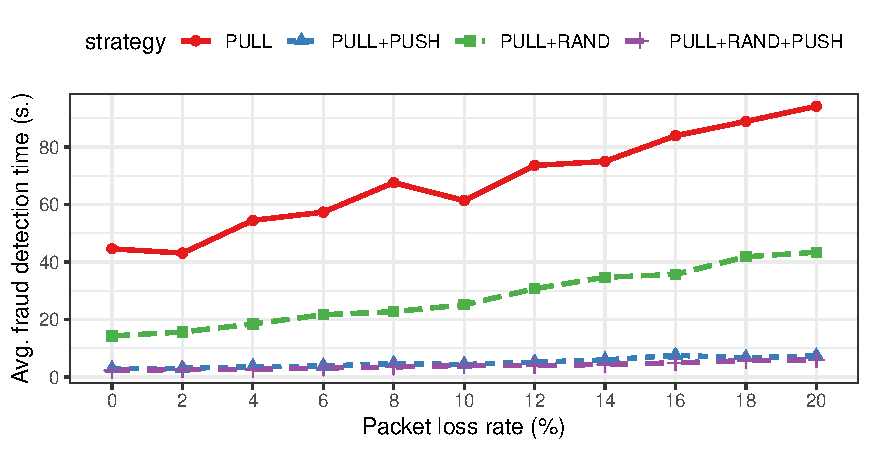
\includegraphics[width=.8\linewidth]{trustchain/assets/fraud_times_send_failure}
	\caption{The effect of packet loss on the average fraud detection times, for different record exchange strategies.}
	\label{fig:fraud_times_link_failures}
\end{figure}

\subsection{Packet Loss}
We reveal the robustness of \TrustChain{} by quantifying the effect of packet loss on the efficiency of fraud detection.
To this end, we increase the packet loss rate, up to 20\%, and run our simulations under our four record exchange strategies.
Even though a packet loss rate of 20\% is unlikely for any environment in which \TrustChain{} is to be deployed, we want to estimate how robust \TrustChain{} is, even in such extreme circumstances.
We expect fraud detection times to increase when network stability is lower since losing packets makes it less likely to detect inconsistencies.

Figure~\ref{fig:fraud_times_link_failures} shows the average fraud detection times when increasing the packet loss rate for our four record exchange strategies.
We observe that fraud detection times increase under the \texttt{PULL} and \texttt{PULL+RAND} strategies, whereas this effect is less for the \texttt{PULL+PUSH} and \texttt{PULL+RAND+PUSH} strategies.
Average fraud detection times, under the \texttt{PULL} strategy, increase from 44.6 seconds with no packet loss to 94.1 seconds when 20\% packet loss.
For the \texttt{PULL+RAND+PUSH} strategy, this same increase is from 2.3 seconds to 6.0 seconds.
We notice that with a packet loss of 20\% and the \texttt{PULL} strategy, 23.8\% of all fraud attempts remains uncovered after the experiment has ended.
This number is just 0.2\% when no packets are lost.
Under the \texttt{PULL+RAND+PUSH} strategy, we see that all fraud attempts are discovered in our experiment, for all evaluated packet loss rates.

\begin{figure}[t]
	\centering
	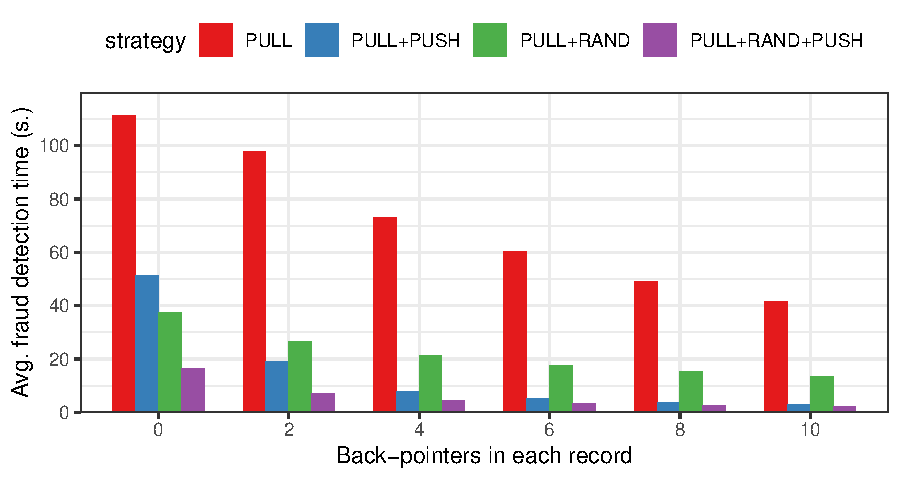
\includegraphics[width=.9\linewidth]{trustchain/assets/fraud_times_back_pointers}
	\caption{The effect of adding more back-pointers to each record on the average fraud detection times, for different record exchange strategies.}
	\label{fig:fraud_times_back_pointers}
\end{figure}

\begin{figure*}[t]
	\centering
	\begin{subfigure}{.8\columnwidth}
		\centering
		
\includegraphics[width=.9\linewidth]{trustchain/assets/fraud_experiments_legend}
	\end{subfigure}
	\begin{subfigure}{.5\columnwidth}
		\centering
		\captionsetup{width=.9\linewidth}
		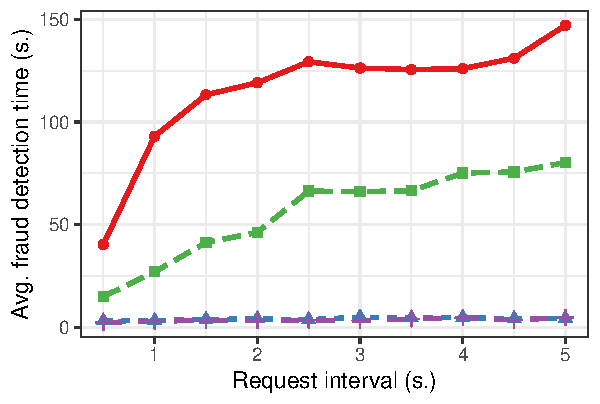
\includegraphics[width=\linewidth]{trustchain/assets/fraud_times_crawl_interval}
		\caption{Average fraud detection times as the request interval increases.}
		\label{fig:experiment_crawl_interval_detection_times}
	\end{subfigure}%
	\begin{subfigure}{.5\columnwidth}
		\centering
		\captionsetup{width=.9\linewidth}
		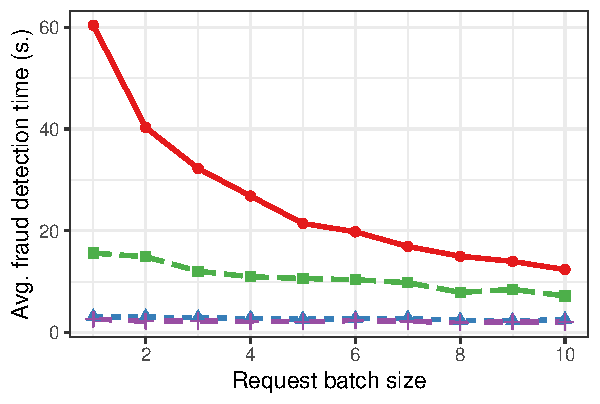
\includegraphics[width=\columnwidth]{trustchain/assets/fraud_times_crawl_batch_size}
		\caption{Average fraud detection times as the request batch size increases.}
		\label{fig:experiment_crawl_batch_size_detection_times}
	\end{subfigure}
	\caption{The effect of changing the request interval batch size on the average fraud detection times.}
	\label{fig:crawl_experiments}
\end{figure*}

\subsection{Request Interval and Batch Size}
We modify the record request interval and batch size and analyse the effect on the average fraud detection times, see Figure~\ref{fig:crawl_experiments}.
Figure~\ref{fig:experiment_crawl_interval_detection_times} visualises the impact of the record request interval on the average fraud detection times for different record exchange strategies.
We increase the record request interval, ranging from 0.5 seconds to 5 seconds, in steps of 0.5 seconds.
First, we observe that the average fraud detection times for the \texttt{PULL+PUSH} and \texttt{PULL+RAND+PUSH} strategies remains roughly constant.
This trend indicates that pushing records to random peers is the dominant logic of the record exchange strategy, very effectively exposing fraud instances.
We also note that average fraud detection times for the \texttt{PULL} and \texttt{PULL+RAND} strategies are increasing when the record request interval becomes larger.
For the \texttt{PULL} strategy, we notice that when the request interval is over 3 seconds, most fraud instances remain undetected after our experiment finishes.
These fraud instances become increasingly harder to detect as the modified record in a personal ledger gets \enquote{buried} under additional records.
As such, the average fraud detection time is likely higher when running the experiment until all fraud instances have been detected.
Unfortunately, we are unable to significantly prolong the experiment duration as our simulations are already using peak memory usage, despite various optimization efforts.

Figure~\ref{fig:experiment_crawl_batch_size_detection_times} shows the average fraud detection times when increasing the number of records queried in each request from 1 to 10, for different record exchange strategies.
Again, the \texttt{PULL+PUSH} and \texttt{PULL+RAND+PUSH} strategies are indifferent to this increase.
The average fraud detection time for the \texttt{PULL} strategy decreases from 60.4 seconds to 12.4 seconds when increasing the request batch size from 1 record to 10 records, respectively.
This decrease indicates that increasing the request batch size is particularly effective when using the \texttt{PULL} strategy, at the expanse of increased bandwidth usage.

\subsection{Back-Pointers}
We vary the number of back-pointers ($ b $) in each record and analyse the effect on average fraud detection times.
We suspect that adding more back-pointers increases the probability of detecting fraud since individual records now bear more hashes of records in ones personal ledger.
This advantage comes, however, at a cost of additional network usage and computational overhead to analyse the back-pointers.
Each back-pointer adds 32 bytes to the serialized record size.

Figure~\ref{fig:fraud_times_back_pointers} shows the average time until fraud is detected while varying the number of back-pointers and considering different record exchange strategies.
Adding additional back-pointers indeed decreases fraud detection times.
Under the \texttt{PULL} record exchange strategy, it takes 111.2 seconds to detect fraud when no additional back-pointers are included. In comparison, this number decreases to 41.6 seconds when adding up to ten back-pointers to each record (a decrease of 58.4\%).
This decrease is much more for the \texttt{PULL+PUSH} strategy, namely 97\%.
Note that the effect of adding more back-pointers diminishes for $ b > 4 $.
This effect can likely be attributed to the fact that all peers start with an empty personal ledger in our simulations, and that different records with lower sequence numbers in the same personal ledger are more likely to include identical hashes in their back-pointers.
However, we believe that the effect of additional back-pointers becomes more apparent when personal ledgers grow to considerable sizes, since different records are then more likely to include more unique hashes.

\begin{figure}[t]
	\centering
	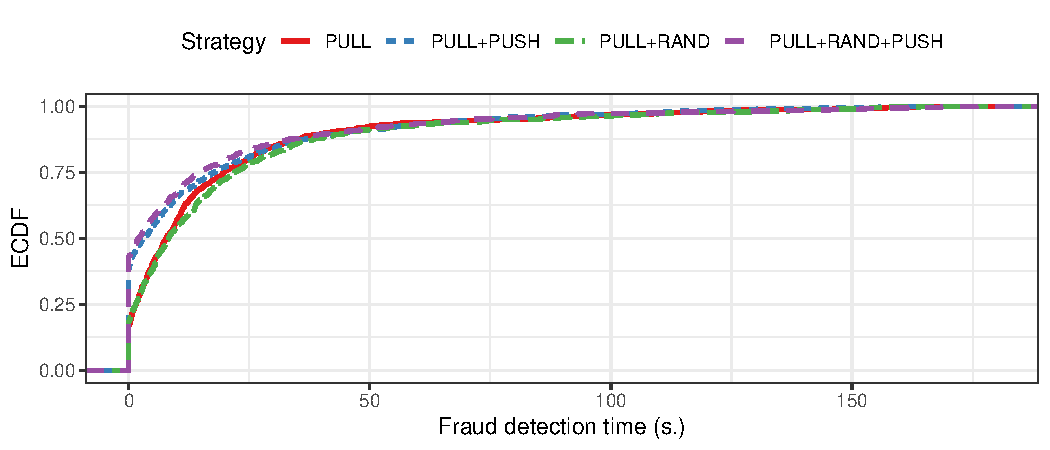
\includegraphics[width=\linewidth]{trustchain/assets/fraud_experiment_realistic_ecdf}
	\caption{Fraud detection times lower than 180 seconds for different record exchange strategies when replaying a day of interactions made by \Tribler{} users.}
	\label{fig:fraud_times_realistic_dataset}
\end{figure}

\subsection{Fraud Detection Times under a Realistic Workload}
\label{subsec:realistic_workload}
Our experiments conducted so far are using a synthetic workload.
We now evaluate the effectiveness of fraud detection in \TrustChain{} of our four considered record exchange strategies using a realistic workload.
This workload is derived from deployment data of \TrustChain{} in \Tribler{}, our decentralized file-sharing application.
An interaction describes network communication between two peers in a Tor-like overlay.
We provide further details on this dataset in Section~\ref{sec:deployment}.
The following experiment replays interactions made during the busiest 24 hours of our deployment period: November 28, 2020.
On this particular day, a total of 440'130 records have been created, involving 2'027 digital identities.
In the following experiment, we simulate a peer for each digital identity.
In line with our prior experiments, each peer commits fraud with a probability of 10\% when creating a new record.
To match the \TrustChain{} settings in our deployed environment (see Section~\ref{sec:deployment}), we increase the record request interval to 10 seconds.

We noticed that all fraud instances have been detected after our experiment ends.
The average fraud detection time for the \texttt{PULL} strategy is just 29.4 seconds whereas this number decreases to 18.5 seconds for the \texttt{PULL+RAND+PUSH} strategy.
2.5\% of all fraud instances take longer than three minutes to detect, with the highest detection time being 1'276 seconds (just over 21 minutes).
Figure~\ref{fig:fraud_times_realistic_dataset} shows the Empirical Cumulative Distribution Function (ECDF) of fraud detection times, for the evaluated strategies.
For presentation clarity, we only show the detection times of fraud instances lower than three minutes.
We observe that over 25\% of all fraud for the \texttt{PULL+PUSH} strategy is detected immediately.
During this experiment, we also see that the network usage per peer is relatively low.
For the \texttt{PULL} strategy, each peer, on average, consumes merely 1.7 MB of hourly network traffic.
This number increases to 5.1 MB under the \texttt{PULL+RAND+PUSH} strategy.

This experiment shows that \TrustChain{}, under a realistic workload of \Tribler{} interactions, exhibit relatively low fraud detection times and has low network usage.
As we have also measured during our deployment trial (see Section~\ref{sec:deployment}), the resource overhead of \TrustChain{} is minimal.
For \Tribler{}, the fraud detection times shown in Figure~\ref{fig:fraud_times_realistic_dataset} are acceptable.
However, as we have also shown in our other experiments, these detection times can further be improved with more frequent record crawling.

\subsection{Discussion}
In summary, our experiments demonstrate that \TrustChain{} exhibits low fraud detection times, scales when the network grows, has reasonable bandwidth overhead, and is robust against packet loss.
We have also demonstrated the effect of the number of back-pointers in each record on the efficiency of fraud detection.
Finally, we have shown that \TrustChain{} remains effective at detecting fraud when using a realistic workload.
Even though we have not evaluated the effect of all parameters in Table~\ref{tab:experiment_parameters}, we believe that this set of experiments provides a good starting point for system designers to adopt and configure \TrustChain{}.
With our open-source simulator, system designers can quickly analyse the effect of different parameters, guided by a synthetic or realistic workload that resembles the behaviour in their application.

We have demonstrated that there is a trade-off between the average fraud detection times and network usage.
The acceptable network usage differs per applications.
For example, bandwidth is less likely to be a bottleneck when considering a video streaming application compared to an Internet-of-Things environment with low-resource devices.
By reducing the record request intervals, fanout value, and the maximum number of back-pointers, one can reduce the bandwidth footprint of \TrustChain{}, at the cost of increased fraud detection times.
Figure~\ref{fig:experiment_scalability_bandwidth} shows that the active record exchange strategy has a notable impact on network usage.
In a dynamic network where the sessions of peers are short-lived, we recommend the \texttt{PULL+RAND} or \texttt{PULL+RAND+PUSH} strategies, where peers share random records in their database with others.
This strategy allows the detection of fraud attempts of offline peers.
We recommend the \texttt{PULL+RAND+PUSH} strategy when fraud must  be detected quickly.
We recommend the \texttt{PULL} strategy when bandwidth is a limiting factor.

\section{Applying \TrustChain{} to Address Free-riding at Scale}
\label{sec:deployment}
To show the effectiveness of \TrustChain{} with a real-world application, we conduct a large-scale deployment trial of \TrustChain{} with \Tribler{}.
\Tribler{} is our decentralized file-sharing application and is downloaded by over 1.8 million users~\cite{pouwelse2008tribler}.
This application features an onion-routing overlay that tunnels BitTorrent traffic through \emph{relay and exit nodes} to provide anonymity.
Unfortunately, the \Tribler{} network suffers from an undersupply of exit nodes, leading to frequent network congestions and overall degradation of download speeds for all users.
We employ \TrustChain{} to account the performed work by relay and exit nodes, and the consumed work by downloaders.
We then punish free-riding behaviour by offering users with higher net contributions preferential treatment during periods of congestion.
In the remainder of this section, we elaborate on the integration of \TrustChain{} in Tribler, on the collected data, and on the effectiveness of free-riding detection.

\begin{figure}[t]
	\centering
	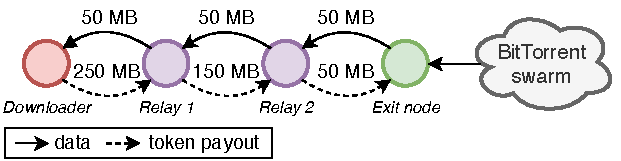
\includegraphics[width=.8\linewidth]{trustchain/assets/payouts}
	\caption{Accounting specifications of an anonymous 50 MB BitTorrent download over a three-hop onion-routing circuit.}
	\label{fig:payouts}
\end{figure}

\subsection{Accounting Bandwidth Transfers}
We enable peers to earn \emph{bandwidth tokens} by providing services as a relay or exit node in the \Tribler{} network.
The mutations in bandwidth token balances of each peer is accounted in \TrustChain{} records.
For example, a payout corresponding to a data exchange of a 50 MB file between peers $ a $ and $ b $ deduces 50 MB of $ a $'s balance and increments $ b $'s balance by 50 MB (MB is the unit of this bandwidth token).
Peers can have a negative balance of bandwidth tokens, in which case they have received more traffic than they contributed to the network.

When a peer downloads content using \Tribler{}, the \Tribler{} software establishes a \emph{circuit}, containing exactly one exit node and optionally some relay nodes.
This is comparable to circuits in the Tor protocol.
All traffic is securely routed through relay and exit nodes.
Figure~\ref{fig:payouts} shows how bandwidth tokens are paid out after a peer has downloaded a 50 MB file over a three-hop circuit (with two relay nodes and one exit node).
The downloader accounts a transfer of 250 MB to the first relay using \TrustChain{}.
Specifically, the downloader creates a proposal record, containing the pair-wise byte counter with the first relay and the magnitude of the current payout.
In the latest version of \Tribler{}, newly created records are by default disseminated to 20 random peers.
Each peer also requests a random record from another known peer every 10 seconds.
During our deployment period, we have periodically revised the record exchange strategy in response to the network behaviour and growth.

After the downloader has finished the payout to the first relay, the first relay then transfers 150 MB to the next relay, resulting in a net positive token balance of 100 MB for the first relay.
The rationale behind our payout scheme is that we reward relay and exit nodes for performing the cryptographic operations on the forwarded data.
Relays that do not forward the payout to the next hop will be added to the local blacklist by the previous hop, therefore lowering their opportunity to earn bandwidth tokens.
%The payload in \TrustChain{} records contains both the token amount transferred and the current token balance of the peer.

Since this use-case involves anonymous downloading, there is an important trade-off between accountability and anonymity.
We plan to address privacy concerns around the accounting of bandwidth transfers by having each peer aggregate and delay payouts.
This privacy-enhancing technique is introduced in the work of Palmieri et al.~\cite{palmieri2015paying}.
Still, work accounting with \TrustChain{} does not leak the identity of a downloader to other peers in the network, nor reveals any data being transferred over circuits.
To address the uncontrolled minting of bandwidth tokens by accounting fake work, we are currently looking into the design and deployment of a Sybil-resistant reputation mechanism~\cite{otte2017trustchain}.

\begin{algorithm}[!t]
	\caption{The assignment logic of slots to circuits. \emph{numRand} and \emph{numComp} represent the maximum number of random and competitive slots, respectively.}
	\label{alg:slot_logic}
	\begin{algorithmic}[1]
		\State randomSlots $ \leftarrow [\bot] * $ numRand
		\State competitiveSlots $ \leftarrow [(-\infty, \bot)] * $ numComp
		\State
		
		\Function{onCircuitRequest}{circuit}
		\For{$ i = 0 $ to numRand}
		\If{randomSlots$[i] = \bot $}
		\State randomSlots$[i] \leftarrow $ circuit
		\State \Return
		\EndIf
		\EndFor
		
		\State Query the balance of the initiator of the circuit
		
		\EndFunction
		\State
		
		\Function{onBalance}{circuit, balance}
		\State lowestBalance $ \leftarrow \infty $
		\State lowestIndex $ \leftarrow \infty $
		\For{$ i = 0 $ to numComp}
		\If{competitiveSlots$[i] = (-\infty, \bot) $}
		\State competitiveSlots$[i] \leftarrow $ (circuit, balance)
		\State \Return
		\EndIf
		
		\If{competitiveSlots$[i][0] < $ lowestBalance}
		\State lowestBalance $ \leftarrow $ competitiveSlots$[i][0] $
		\State lowestIndex $ \leftarrow i $
		\EndIf
		\EndFor
		
		\If{balance $ > $ lowestBalance}
		\State \textsc{destroyCircuit}(competitiveSlots$[$lowestIndex$][1] $)
		\State competitiveSlots$[$lowestIndex$] \leftarrow $ (circuit, balance)
		\EndIf
		
		\EndFunction
		
	\end{algorithmic}
\end{algorithm}

\subsection{Circuit Assignment}
We use the bandwidth token balances included in \TrustChain{} records to grant preferential treatment to dedicated peers during periods of congestion.
Specifically, we modify the \Tribler{} protocol such that each relay and exit nodes maintain a fixed number of \emph{slots}.
A circuit that includes a relay or exit nodes consumes one slot at their side.
We distinguish between \emph{random} and \emph{competitive} slots.
Random slots are filled on a first-come-first-serve basis whereas the assignment of competitive slot is based on the bandwidth token balance of a circuit initiator.
The intuition behind this approach is to still give peers with lower trust scores an opportunity to earn a (random) slot but at the same time, give preferential treatment to well-behaving peers with competitive slots.
The total number of such slots can be changed, depending on the hardware capabilities of the node operator.

A pseudocode description of the slot assignment logic is given in Listing~\ref{alg:slot_logic}.
When a circuit initiation request arrives, the \texttt{onCircuitRequest} method is invoked and \Tribler{} first determines if there is a random slot available (line 5-9).
If so, we assign the new circuit to the random slot (line 7).
If no random slot is available, \Tribler{} queries the bandwidth token balance of the circuit initiator $ i $ by requesting the records in the personal ledger of $ i $.
When receiving these records, \Tribler{} determines the current bandwidth token balance and checks eligibility for a competitive slot (line 12-23).
If there is an unoccupied competitive slot, \Tribler{} assigns the new circuit to it (line 16).
If all competitive slots are filled, the circuit of the initiator with the lowest amount of bandwidth tokens, say $ p $, is destroyed if the token balance of $ i $ is higher than the token balance of $ p $ (line 22).
This pre-emptive approach frees up the competitive slot for the circuit of $ i $.
As a result, users with a higher token balance have more chance to claim a competitive slot during periods of congestion, compared to free-riders, and experience higher and more stable download speeds.
We consider the analysis of different allocation policies, e.g., using a packet-granular scheduler~\cite{jansen2018kist}, as further work.

%\begin{figure}[t]
%	\centering
%	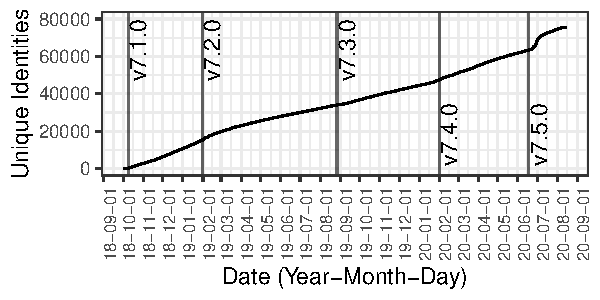
\includegraphics[width=\linewidth]{assets/identities_per_day}
%	\caption{ECDF showing the distribution of bandwidth token balances users and individual rejects events at exit nodes.}
%	\label{fig:identities_per_day}
%\end{figure}

\begin{figure}[!t]
	\centering
	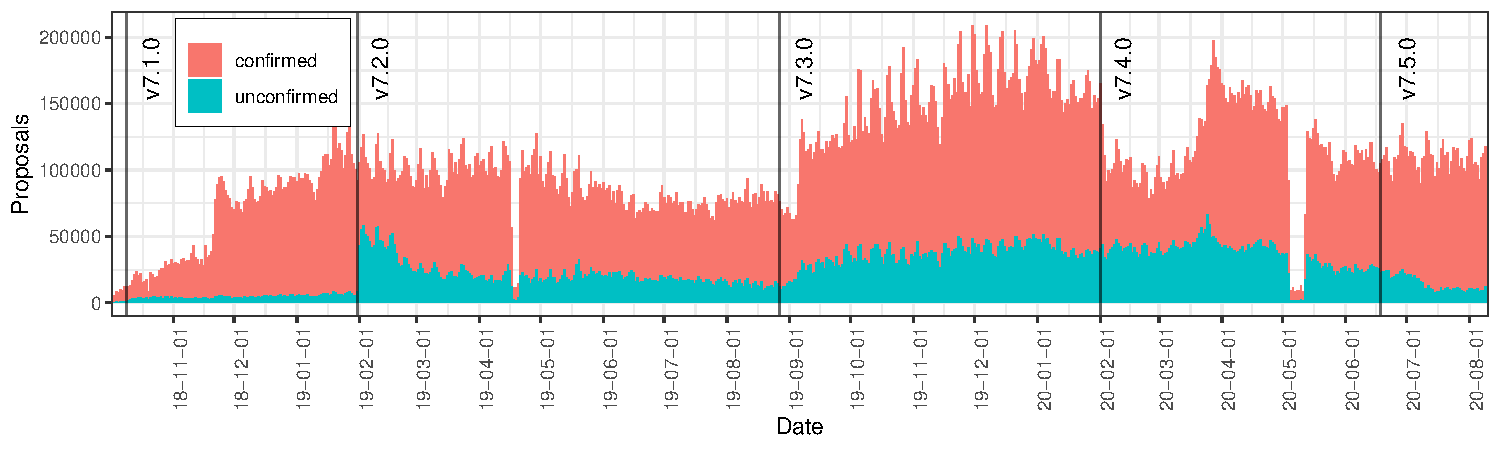
\includegraphics[width=\linewidth]{trustchain/assets/record_creation}
	\caption{Daily creation statistics of proposals, during our two-year deployment trial. We show the amount of confirmed and unconfirmed proposals. We annotate the major releases of \Tribler{}.}
	\label{fig:record_creation}
\end{figure}

\subsection{Data Collection}
We integrate both \TrustChain{} and the slot assignment logic in \Tribler{} and release a new version of our software.
We also deploy a crawler that continuously requests \TrustChain{} records from random peers in the \Tribler{} network.
This crawler selects a random peer in the \TrustChain{} network every two seconds and requests missing records in their personal ledger.
The crawler statistics are published on a public website.\footnote{See \url{http://explorer.tribler.org}}
A deployment period of two years has resulted in more than \TrialRecords{} records, created by over \TrialUsers{} peers.
The crawler stores collected records in a sqlite database that is enhanced with additional indices to speed up insertion and analysis queries.
The file size of the database with all collected records is around 120GB, and we plan on releasing the full data set later.
Our crawler discovered 127'135 proofs of fraud.
We also find that 11.4\% of all collected proposals in the deployed \TrustChain{} network is unconfirmed.
This fraction of unconfirmed proposals is either because the proposal counterparty has not created a confirmation, or because our crawler has not picked up the confirmation record.

Deploying a crawler and monitoring the records created by \TrustChain{} allows us to detect anomalies caused by software bugs or unexpected user behaviour.
It also provides us with the means to monitor the growth of users within \Tribler{} by tracking the number of unique peers in the \TrustChain{} network.
We have also included a creation timestamp in the payload of each record created with \Tribler{}, allowing us to perform a time-based analysis.

Figure~\ref{fig:record_creation} shows the daily number of created proposal records.
We annotate the dates on which we released a major version of \Tribler{}.
Figure~\ref{fig:record_creation} reveals that more users run \Tribler{} during the weekend and create more proposals on a Saturday and a Sunday.
We also observed two large-scale outage of exit nodes, in April 2019 and May 2020, likely due to infrastructure failures.
Despite these outages, users would still perform payouts when downloading directly from other \Tribler{} users without anonymity.

%In \Tribler{}, users earn bandwidth tokens by either operating an exit node, or by relaying traffic.
%By default, users download with one-hop anonymity, meaning that the circuit is directly connected to an available exit node.
%We noticed that only few users increase this setting since adding additional hops to a circuit negatively impacts the achievable download speed.
%There is a delicate trade-off between anonymity and download speed. 
%Therefore, there is an oversupply of relay nodes but the majority of users do not require a relay node for their downloads.
%Eventually, we aim to adjust the default number of hops for a download to two, increasing the opportunities for relay nodes to earn bandwidth tokens.
%We are currently improving the performance of our anonymous download mechanism.

\begin{figure}[t]
	\centering
	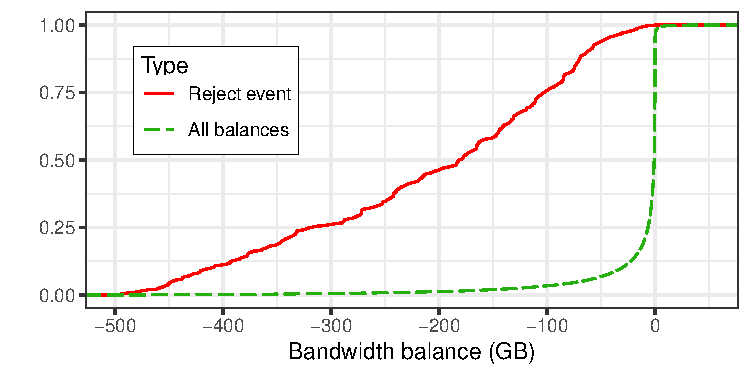
\includegraphics[width=.8\linewidth]{trustchain/assets/exit_node_rejects}
	\caption{Emperical Cumulative Distribution Function (ECDF) of the bandwidth token balances of peers and individual rejects events at exit nodes.}
	\label{fig:exit_node_rejects}
\end{figure}

\subsection{Free-rider Identification and Service Refusal}
To show the effect of \TrustChain{} and our slot assignment mechanism on free riders, we deploy 48 exit nodes in the \Tribler{} network, running on the same machine.
Each exit node is configured with a total of 10 random slots and 20 competitive slots, resulting in a total of 1'440 slots.
We determined this number of random and competitive slots based on the hardware capacity of our machine.
We are specifically interested in the situation when a peer is unable to claim a slot, due to their bandwidth token balance being insufficient.
We refer to this situation as a \emph{reject event}.
For each reject event, we log the bandwidth token balance of the rejected peer.
In total, we logged over 1.4 million reject events over three weeks.

Figure~\ref{fig:exit_node_rejects} shows an Empirical Cumulative Distribution Function (ECDF) with the bandwidth token balances of all peers (dotted green line) and the balances associated with rejected circuit requests (solid red line).
For presentation clarity, we filter out all peers and reject events with balances higher than 50GB or lower than -500GB.
Many Tribler users have a negative bandwidth token balance.
The median token balance of all users is -713 MB.
This number suggests that there is not much opportunity to earn bandwidth tokens by contributing to the network.
By default, the Tribler software downloads content over a 1-hop circuit, only involving an exit node.
Changing the default behaviour to use 2-hop downloads could alleviate this issue, at the cost of decreased download speeds.
Figure~\ref{fig:exit_node_rejects} also shows that users with a relatively low (e.g., $ < $ 50 GB) are frequently rejected a slot.
The median token balance associated with reject events is -181.4 GB, demonstrating that our mechanism effectively targets peers with lower bandwidth token balances.
The slots claimed by free-riders will likely go to dedicated peers when the network is congested.
This deployment trial shows that \TrustChain{} is effective at detecting and addressing free-riding behaviour in \Tribler{}.
The integration of \TrustChain{} has increases network performance and helps to maintain fairness amongst downloading users.

%\begin{figure}[t]
%	\centering
%	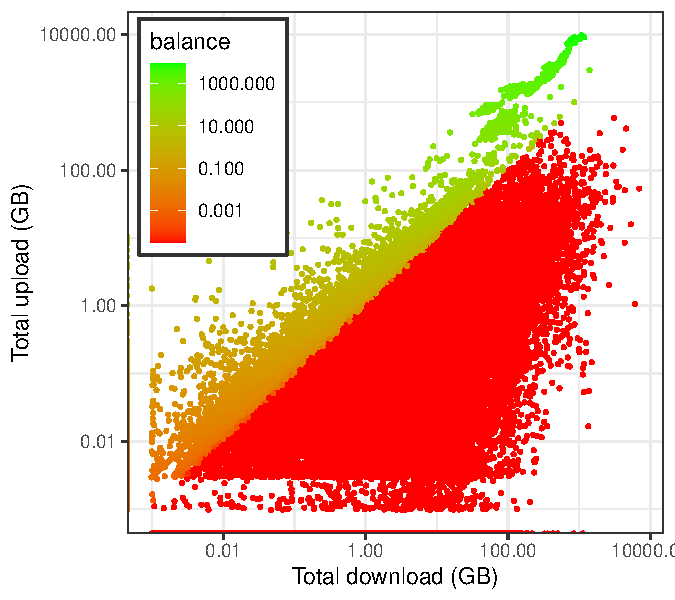
\includegraphics[width=\linewidth]{assets/balances_scatter}
%	\caption{The bandwidth balances of users in Tribler. Users with a balances less than 5GB are marked red.}
%	\label{fig:balances}
%\end{figure}

%\begin{figure}[t]
%	\centering
%	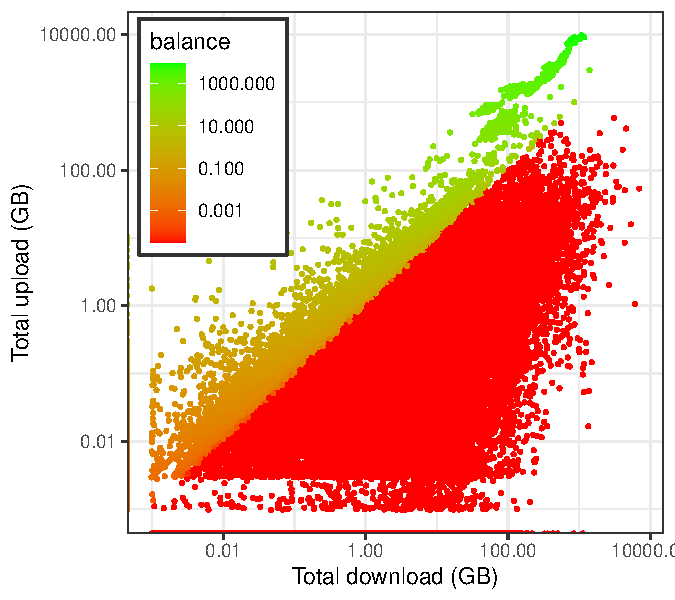
\includegraphics[width=\linewidth]{assets/balances_scatter}
%	\caption{Scatterplot of user balances where each point represents a user in \Tribler{}.}
%	\label{fig:balances_scatter}
%\end{figure}

\section{Conclusions}
We have presented \TrustChain{}, a universal accounting mechanism to maintain fairness in decentralized applications by accounting work.
The \TrustChain{} data structure uses records to capture the work performed by peers.
Each peer maintains a tamper-evident personal ledger with interlinked records.
Fraud, the illegitimate modification of a record in ones personal ledger, is optimistically detected through the random exchange of records and thorough validation of incoming ones.
We have devised a system architecture of \TrustChain{} and implemented it.
Our evaluation has demonstrated that \TrustChain{} is capable of detecting fraud within seconds, even when the network grows to 10'000 peers and when scaling the system load.
Through a two-year deployment trial of \TrustChain{} in \Tribler{}, involving more than \TrialUsers{} users, we have successfully addressed free-riding behaviour.

We envision and encourage the usage of \TrustChain{} beyond work accounting in decentralized applications.
Currently, \TrustChain{} is being evaluated in different scenarios that require accountability, including decentralized trading, software developer portfolios, and self-sovereign identity~\cite{de2021xchange,de2019devid,stokkink2018deployment}.